\documentclass[11pt]{article}

% The four macros of the header standard; tools/zenodo/publish_revision.py patches them when it reserves the DOI.
\newcommand{\doctype}{Preprint}
\newcommand{\docversion}{v1.00.000}
\newcommand{\docdate}{8 November 2026}
\newcommand{\versiondoi}{10.5281/zenodo.24053168}
\newcommand{\conceptdoi}{10.5281/zenodo.24053167}
\newcommand{\docidentity}{CAOS\_Contraste, the validation of the risk models of a bank}

% The packages and conventions every Contraste manuscript shares (CAOS_MANAGE conventions/manuscript-content-bar.md
% section 2). A document sets its class, the four header macros and \docidentity, then % The packages and conventions every Contraste manuscript shares (CAOS_MANAGE conventions/manuscript-content-bar.md
% section 2). A document sets its class, the four header macros and \docidentity, then % The packages and conventions every Contraste manuscript shares (CAOS_MANAGE conventions/manuscript-content-bar.md
% section 2). A document sets its class, the four header macros and \docidentity, then \input{../_shared/preamble}.
\usepackage[T1]{fontenc}
\usepackage[utf8]{inputenc}
\usepackage{lmodern}
\usepackage{microtype}
\usepackage[a4paper,margin=2.5cm]{geometry}
\usepackage{amsmath,amssymb,amsthm,mathtools,bm}
\usepackage{graphicx}
\usepackage{booktabs,longtable,tabularx,array,multirow}
\usepackage{siunitx}
\usepackage{algorithm}
\usepackage{algpseudocode}
\usepackage{caption,subcaption}
\usepackage{xcolor}
\usepackage[numbers,sort&compress]{natbib}
\usepackage[hidelinks]{hyperref}
\usepackage{cleveref}
\usepackage{orcidlink}

\sisetup{group-separator={,},group-minimum-digits=4,detect-all}
\graphicspath{{figures/}{../figures/}}
\captionsetup{font=small,labelfont=bf}
\setlength{\LTcapwidth}{\textwidth}

% Theorem environments for the Theory sections of the manuscripts.
\newtheorem{proposition}{Proposition}
\newtheorem{lemma}{Lemma}
\newtheorem{corollary}{Corollary}
\theoremstyle{definition}
\newtheorem{definition}{Definition}
\newtheorem{assumption}{Assumption}
\theoremstyle{remark}
\newtheorem{remark}{Remark}

% Notation shared by the documents (each defines it again in its notation table).
\newcommand{\E}{\mathbb{E}}
\newcommand{\Prob}{\mathbb{P}}
\newcommand{\Var}{\operatorname{Var}}
\newcommand{\Cov}{\operatorname{Cov}}
\newcommand{\VaR}{\operatorname{VaR}}
\newcommand{\ES}{\operatorname{ES}}
\newcommand{\PD}{\mathrm{PD}}
\newcommand{\LGD}{\mathrm{LGD}}
\newcommand{\EAD}{\mathrm{EAD}}
\newcommand{\ECL}{\mathrm{ECL}}
\newcommand{\indic}{\mathbf{1}}
\newcommand{\R}{\mathbb{R}}
\newcommand{\dd}{\,\mathrm{d}}

% The page-1 header block (CAOS_MANAGE conventions/manuscript-header-standard.md). The document defines \doctype,
% \docversion, \docdate, \versiondoi, \conceptdoi and \docidentity before this file; the publishing tool patches the four
% macros of the standard when it reserves the version DOI.
\newcommand{\docrepo}{github.com/fsantibanezleal/CAOS\_Contraste}
\newcommand{\headerblock}{%
\begin{center}
\fbox{\parbox{0.94\textwidth}{\small\raggedright
\textbf{\doctype} \quad$\cdot$\quad \docversion, \docdate \quad$\cdot$\quad Licence CC BY 4.0\\[2pt]
CAOS open-research programme \quad$\cdot$\quad \docidentity\\[2pt]
Version DOI \href{https://doi.org/\versiondoi}{\texttt{\versiondoi}} \quad$\cdot$\quad
concept DOI (always latest) \href{https://doi.org/\conceptdoi}{\texttt{\conceptdoi}}\\[2pt]
Not peer reviewed. Source code, data and computational records: \href{https://\docrepo}{\texttt{\docrepo}}
}}
\end{center}
\vspace{4pt}}
.
\usepackage[T1]{fontenc}
\usepackage[utf8]{inputenc}
\usepackage{lmodern}
\usepackage{microtype}
\usepackage[a4paper,margin=2.5cm]{geometry}
\usepackage{amsmath,amssymb,amsthm,mathtools,bm}
\usepackage{graphicx}
\usepackage{booktabs,longtable,tabularx,array,multirow}
\usepackage{siunitx}
\usepackage{algorithm}
\usepackage{algpseudocode}
\usepackage{caption,subcaption}
\usepackage{xcolor}
\usepackage[numbers,sort&compress]{natbib}
\usepackage[hidelinks]{hyperref}
\usepackage{cleveref}
\usepackage{orcidlink}

\sisetup{group-separator={,},group-minimum-digits=4,detect-all}
\graphicspath{{figures/}{../figures/}}
\captionsetup{font=small,labelfont=bf}
\setlength{\LTcapwidth}{\textwidth}

% Theorem environments for the Theory sections of the manuscripts.
\newtheorem{proposition}{Proposition}
\newtheorem{lemma}{Lemma}
\newtheorem{corollary}{Corollary}
\theoremstyle{definition}
\newtheorem{definition}{Definition}
\newtheorem{assumption}{Assumption}
\theoremstyle{remark}
\newtheorem{remark}{Remark}

% Notation shared by the documents (each defines it again in its notation table).
\newcommand{\E}{\mathbb{E}}
\newcommand{\Prob}{\mathbb{P}}
\newcommand{\Var}{\operatorname{Var}}
\newcommand{\Cov}{\operatorname{Cov}}
\newcommand{\VaR}{\operatorname{VaR}}
\newcommand{\ES}{\operatorname{ES}}
\newcommand{\PD}{\mathrm{PD}}
\newcommand{\LGD}{\mathrm{LGD}}
\newcommand{\EAD}{\mathrm{EAD}}
\newcommand{\ECL}{\mathrm{ECL}}
\newcommand{\indic}{\mathbf{1}}
\newcommand{\R}{\mathbb{R}}
\newcommand{\dd}{\,\mathrm{d}}

% The page-1 header block (CAOS_MANAGE conventions/manuscript-header-standard.md). The document defines \doctype,
% \docversion, \docdate, \versiondoi, \conceptdoi and \docidentity before this file; the publishing tool patches the four
% macros of the standard when it reserves the version DOI.
\newcommand{\docrepo}{github.com/fsantibanezleal/CAOS\_Contraste}
\newcommand{\headerblock}{%
\begin{center}
\fbox{\parbox{0.94\textwidth}{\small\raggedright
\textbf{\doctype} \quad$\cdot$\quad \docversion, \docdate \quad$\cdot$\quad Licence CC BY 4.0\\[2pt]
CAOS open-research programme \quad$\cdot$\quad \docidentity\\[2pt]
Version DOI \href{https://doi.org/\versiondoi}{\texttt{\versiondoi}} \quad$\cdot$\quad
concept DOI (always latest) \href{https://doi.org/\conceptdoi}{\texttt{\conceptdoi}}\\[2pt]
Not peer reviewed. Source code, data and computational records: \href{https://\docrepo}{\texttt{\docrepo}}
}}
\end{center}
\vspace{4pt}}
.
\usepackage[T1]{fontenc}
\usepackage[utf8]{inputenc}
\usepackage{lmodern}
\usepackage{microtype}
\usepackage[a4paper,margin=2.5cm]{geometry}
\usepackage{amsmath,amssymb,amsthm,mathtools,bm}
\usepackage{graphicx}
\usepackage{booktabs,longtable,tabularx,array,multirow}
\usepackage{siunitx}
\usepackage{algorithm}
\usepackage{algpseudocode}
\usepackage{caption,subcaption}
\usepackage{xcolor}
\usepackage[numbers,sort&compress]{natbib}
\usepackage[hidelinks]{hyperref}
\usepackage{cleveref}
\usepackage{orcidlink}

\sisetup{group-separator={,},group-minimum-digits=4,detect-all}
\graphicspath{{figures/}{../figures/}}
\captionsetup{font=small,labelfont=bf}
\setlength{\LTcapwidth}{\textwidth}

% Theorem environments for the Theory sections of the manuscripts.
\newtheorem{proposition}{Proposition}
\newtheorem{lemma}{Lemma}
\newtheorem{corollary}{Corollary}
\theoremstyle{definition}
\newtheorem{definition}{Definition}
\newtheorem{assumption}{Assumption}
\theoremstyle{remark}
\newtheorem{remark}{Remark}

% Notation shared by the documents (each defines it again in its notation table).
\newcommand{\E}{\mathbb{E}}
\newcommand{\Prob}{\mathbb{P}}
\newcommand{\Var}{\operatorname{Var}}
\newcommand{\Cov}{\operatorname{Cov}}
\newcommand{\VaR}{\operatorname{VaR}}
\newcommand{\ES}{\operatorname{ES}}
\newcommand{\PD}{\mathrm{PD}}
\newcommand{\LGD}{\mathrm{LGD}}
\newcommand{\EAD}{\mathrm{EAD}}
\newcommand{\ECL}{\mathrm{ECL}}
\newcommand{\indic}{\mathbf{1}}
\newcommand{\R}{\mathbb{R}}
\newcommand{\dd}{\,\mathrm{d}}

% The page-1 header block (CAOS_MANAGE conventions/manuscript-header-standard.md). The document defines \doctype,
% \docversion, \docdate, \versiondoi, \conceptdoi and \docidentity before this file; the publishing tool patches the four
% macros of the standard when it reserves the version DOI.
\newcommand{\docrepo}{github.com/fsantibanezleal/CAOS\_Contraste}
\newcommand{\headerblock}{%
\begin{center}
\fbox{\parbox{0.94\textwidth}{\small\raggedright
\textbf{\doctype} \quad$\cdot$\quad \docversion, \docdate \quad$\cdot$\quad Licence CC BY 4.0\\[2pt]
CAOS open-research programme \quad$\cdot$\quad \docidentity\\[2pt]
Version DOI \href{https://doi.org/\versiondoi}{\texttt{\versiondoi}} \quad$\cdot$\quad
concept DOI (always latest) \href{https://doi.org/\conceptdoi}{\texttt{\conceptdoi}}\\[2pt]
Not peer reviewed. Source code, data and computational records: \href{https://\docrepo}{\texttt{\docrepo}}
}}
\end{center}
\vspace{4pt}}


% Every number quoted in the prose is a macro written by make_artifacts.py from the committed documents and the experiment outputs.
% Generated by make_artifacts.py: every number quoted in the prose.
\newcommand{\bdAblBoundsGain}{2}
\newcommand{\bdAblFull}{10}
\newcommand{\bdAblFullWidth}{1.26}
\newcommand{\bdAblGaussPoint}{2}
\newcommand{\bdAblGaussTen}{2}
\newcommand{\bdAblHybridPoint}{5}
\newcommand{\bdAblKendallPoint}{5}
\newcommand{\bdAblNoBounds}{8}
\newcommand{\bdAblNoBoundsWidth}{0.17}
\newcommand{\bdAblNoStress}{2}
\newcommand{\bdAblNoStressWidth}{0.11}
\newcommand{\bdAblNoT}{2}
\newcommand{\bdAblNoTStress}{5}
\newcommand{\bdAblNoTStressWidth}{0.14}
\newcommand{\bdAblNoTWidth}{0.07}
\newcommand{\bdAblStressGain}{6}
\newcommand{\bdAblSumPoint}{0}
\newcommand{\bdAblTOnly}{6}
\newcommand{\bdAblTOnlyWidth}{0.15}
\newcommand{\bdAblVcPoint}{2}
\newcommand{\bdAblWidthBounds}{1.09}
\newcommand{\bdAblWidthStress}{0.07}
\newcommand{\bdAdditiveOver}{33.8}
\newcommand{\bdAggregates}{6}
\newcommand{\bdAm}{67.4}
\newcommand{\bdBandSeconds}{10}
\newcommand{\bdBenefitCredit}{25}
\newcommand{\bdBenefitIrrbb}{26}
\newcommand{\bdBenefitMarket}{22}
\newcommand{\bdBenefitOperational}{47}
\newcommand{\bdBoundsSd}{0.1}
\newcommand{\bdBoundsSeconds}{3}
\newcommand{\bdBracketStat}{704.8}
\newcommand{\bdClaytonTauExact}{0.500}
\newcommand{\bdClaytonTauSim}{0.498}
\newcommand{\bdClaytonTheta}{0.60}
\newcommand{\bdComoVar}{724.9}
\newcommand{\bdCopulaDiffEight}{7.4}
\newcommand{\bdCopulaDiffFour}{12.3}
\newcommand{\bdCopulaDiffThirty}{1.5}
\newcommand{\bdCopulaStat}{12.3}
\newcommand{\bdCovInterior}{2}
\newcommand{\bdCovInteriorStress}{8}
\newcommand{\bdCovSharp}{10}
\newcommand{\bdDistinct}{2}
\newcommand{\bdEcCredit}{260.6}
\newcommand{\bdEcIrrbb}{72.8}
\newcommand{\bdEcMarket}{283.4}
\newcommand{\bdEcOperational}{41.2}
\newcommand{\bdEcShareCredit}{40}
\newcommand{\bdEcShareIrrbb}{11}
\newcommand{\bdEcShareMarket}{43}
\newcommand{\bdEcShareOperational}{6}
\newcommand{\bdElCredit}{37.6}
\newcommand{\bdElIrrbb}{27.9}
\newcommand{\bdElMarket}{0.0}
\newcommand{\bdElOperational}{1.2}
\newcommand{\bdElTotal}{66.7}
\newcommand{\bdEsCredit}{346.9}
\newcommand{\bdEsIrrbb}{106.4}
\newcommand{\bdEsMarket}{355.8}
\newcommand{\bdEsOperational}{171.1}
\newcommand{\bdEsTotal}{709.4}
\newcommand{\bdEsTotalMean}{703.7}
\newcommand{\bdEsTotalSd}{20.71}
\newcommand{\bdEulerGap}{1.6\times 10^{-16}}
\newcommand{\bdEulerMaxGap}{3.3\times 10^{-16}}
\newcommand{\bdFarthestGauss}{76}
\newcommand{\bdFarthestLower}{595}
\newcommand{\bdFarthestMax}{595}
\newcommand{\bdFarthestMin}{76}
\newcommand{\bdFarthestSum}{82}
\newcommand{\bdFarthestVc}{78}
\newcommand{\bdFarthestWorst}{86}
\newcommand{\bdGauss}{492.0}
\newcommand{\bdGaussBelow}{25.2}
\newcommand{\bdGaussDepMax}{20}
\newcommand{\bdGaussDepMin}{11}
\newcommand{\bdGaussDf}{0.748}
\newcommand{\bdGaussErrClaytonSurvival}{-16.3}
\newcommand{\bdGaussErrGaussianBase}{0.0}
\newcommand{\bdGaussErrGaussianCrisis}{-15.3}
\newcommand{\bdGaussErrGaussianIndependent}{39.9}
\newcommand{\bdGaussErrGaussianStress}{-11.4}
\newcommand{\bdGaussErrGumbel}{-15.4}
\newcommand{\bdGaussErrRegimeMixture}{-1.1}
\newcommand{\bdGaussErrTthreeBase}{-12.2}
\newcommand{\bdGaussErrTthreeCrisis}{-20.1}
\newcommand{\bdGaussErrTtwofiveBase}{-13.0}
\newcommand{\bdGaussM}{491{,}974}
\newcommand{\bdGaussMaxErr}{39.9}
\newcommand{\bdGaussMedErr}{14.1}
\newcommand{\bdGaussMove}{12.1}
\newcommand{\bdGaussRelDiff}{0.0051}
\newcommand{\bdGaussSd}{3.2}
\newcommand{\bdGaussStress}{551.6}
\newcommand{\bdGaussStressDf}{0.838}
\newcommand{\bdGaussWithin}{2}
\newcommand{\bdGridPoints}{1{,}961}
\newcommand{\bdGumbelTauExact}{0.400}
\newcommand{\bdGumbelTauSim}{0.394}
\newcommand{\bdGumbelTheta}{1.30}
\newcommand{\bdGxBase}{66.9}
\newcommand{\bdGxEta}{0.05}
\newcommand{\bdGxWorst}{143.2}
\newcommand{\bdHeadline}{658.0}
\newcommand{\bdHeadlineChange}{-17.9}
\newcommand{\bdHeadlineM}{658{,}046}
\newcommand{\bdHybridMaxErr}{17.7}
\newcommand{\bdHybridMedErr}{6.5}
\newcommand{\bdKGaussMax}{1}
\newcommand{\bdKTailMax}{22}
\newcommand{\bdKTailMin}{6}
\newcommand{\bdKendallMaxErr}{21.8}
\newcommand{\bdKendallMedErr}{3.6}
\newcommand{\bdLower}{118.5}
\newcommand{\bdLowerDf}{0.180}
\newcommand{\bdLowerM}{118{,}517}
\newcommand{\bdLowerMove}{0.0}
\newcommand{\bdLowerOverHeadline}{0.180}
\newcommand{\bdLowerRangeHi}{186.2}
\newcommand{\bdLowerRangeLo}{185.2}
\newcommand{\bdLowerRangeWidth}{0.99}
\newcommand{\bdLowerRelDiff}{0.0075}
\newcommand{\bdLowerStress}{118.5}
\newcommand{\bdLowerStressDf}{0.180}
\newcommand{\bdLowerVar}{185.2}
\newcommand{\bdMarketEcChange}{-41}
\newcommand{\bdMarketEcNineNine}{165.9}
\newcommand{\bdMarketGridMin}{-1{,}238.9}
\newcommand{\bdMaxRelDiff}{0.0075}
\newcommand{\bdMaxSd}{4.1}
\newcommand{\bdMaxSe}{3.4}
\newcommand{\bdMissedNoBounds}{Gaussian, independent risks and t copula, 3 degrees, crisis matrix}
\newcommand{\bdNStruct}{10}
\newcommand{\bdNuHundredGap}{2.4}
\newcommand{\bdNuSpanBase}{66.5}
\newcommand{\bdNuSpanPc}{13.4}
\newcommand{\bdRearrCells}{2{,}000}
\newcommand{\bdRearrMaxAfter}{19{,}395.8}
\newcommand{\bdRearrMaxComo}{20{,}669.2}
\newcommand{\bdRearrMinAfter}{890.0}
\newcommand{\bdRearrMinComo}{724.9}
\newcommand{\bdRearrSweeps}{8}
\newcommand{\bdRepsBase}{20}
\newcommand{\bdRepsStress}{10}
\newcommand{\bdRm}{0.470}
\newcommand{\bdRmPct}{47}
\newcommand{\bdRsOver}{33.8}
\newcommand{\bdRunnableGaussOnly}{6}
\newcommand{\bdSaShareCredit}{35.4}
\newcommand{\bdSaShareIrrbb}{10.9}
\newcommand{\bdSaShareMarket}{36.3}
\newcommand{\bdSaShareOperational}{17.5}
\newcommand{\bdShareCredit}{36.7}
\newcommand{\bdShareIrrbb}{11.2}
\newcommand{\bdShareMarket}{39.3}
\newcommand{\bdShareOperational}{12.8}
\newcommand{\bdShareSdCredit}{1.2}
\newcommand{\bdShareSdIrrbb}{0.3}
\newcommand{\bdShareSdMarket}{1.3}
\newcommand{\bdShareSdMax}{2.7}
\newcommand{\bdShareSdMin}{0.3}
\newcommand{\bdShareSdOperational}{2.7}
\newcommand{\bdSlack}{90.2}
\newcommand{\bdSqrtFloor}{394.0}
\newcommand{\bdStandaloneOver}{1.393}
\newcommand{\bdStressStat}{12.1}
\newcommand{\bdSumErrMaxOther}{35}
\newcommand{\bdSumErrMin}{8}
\newcommand{\bdSumEs}{980.2}
\newcommand{\bdSumMaxErr}{88.7}
\newcommand{\bdSumMismatch}{540.5}
\newcommand{\bdSumStandaloneEs}{980.2}
\newcommand{\bdSumVar}{724.8}
\newcommand{\bdSweeps}{4, 4, 10, 10}
\newcommand{\bdTEight}{528.3}
\newcommand{\bdTEightDf}{0.803}
\newcommand{\bdTEightM}{528{,}320}
\newcommand{\bdTEightMove}{9.2}
\newcommand{\bdTEightStress}{577.1}
\newcommand{\bdTEightStressDf}{0.877}
\newcommand{\bdTFour}{552.4}
\newcommand{\bdTFourDf}{0.839}
\newcommand{\bdTFourM}{552{,}389}
\newcommand{\bdTFourMove}{6.4}
\newcommand{\bdTFourSd}{4.1}
\newcommand{\bdTFourStress}{587.5}
\newcommand{\bdTFourStressDf}{0.893}
\newcommand{\bdTHundred}{494.4}
\newcommand{\bdTLambdaFour}{0.253}
\newcommand{\bdTLambdaLowFour}{0.127}
\newcommand{\bdTLambdaThirty}{0.0030}
\newcommand{\bdTLambdaThree}{0.312}
\newcommand{\bdTLambdaTwoFive}{0.349}
\newcommand{\bdTThirty}{499.1}
\newcommand{\bdTThirtyDf}{0.759}
\newcommand{\bdTThirtyM}{499{,}128}
\newcommand{\bdTThirtyMove}{11.6}
\newcommand{\bdTThirtyStress}{557.2}
\newcommand{\bdTThirtyStressDf}{0.847}
\newcommand{\bdTThree}{563.2}
\newcommand{\bdTTwoFive}{560.8}
\newcommand{\bdTauBar}{0.2308}
\newcommand{\bdTestsTotal}{9}
\newcommand{\bdTruthClaytonSurvival}{583.2}
\newcommand{\bdTruthDfClaytonSurvival}{0.886}
\newcommand{\bdTruthDfGaussianBase}{0.741}
\newcommand{\bdTruthDfGaussianCrisis}{0.875}
\newcommand{\bdTruthDfGaussianIndependent}{0.530}
\newcommand{\bdTruthDfGaussianStress}{0.837}
\newcommand{\bdTruthDfGumbel}{0.877}
\newcommand{\bdTruthDfRegimeMixture}{0.750}
\newcommand{\bdTruthDfTthreeBase}{0.844}
\newcommand{\bdTruthDfTthreeCrisis}{0.929}
\newcommand{\bdTruthDfTtwofiveBase}{0.852}
\newcommand{\bdTruthGaussianBase}{487.9}
\newcommand{\bdTruthGaussianCrisis}{575.9}
\newcommand{\bdTruthGaussianIndependent}{348.8}
\newcommand{\bdTruthGaussianStress}{551.1}
\newcommand{\bdTruthGumbel}{577.0}
\newcommand{\bdTruthMax}{611.1}
\newcommand{\bdTruthMaxOverHeadline}{0.929}
\newcommand{\bdTruthMaxOverWorst}{0.742}
\newcommand{\bdTruthMin}{348.8}
\newcommand{\bdTruthRegimeMixture}{493.7}
\newcommand{\bdTruthReps}{20}
\newcommand{\bdTruthSeMax}{1.1}
\newcommand{\bdTruthTthreeBase}{555.6}
\newcommand{\bdTruthTthreeCrisis}{611.1}
\newcommand{\bdTruthTtwofiveBase}{560.9}
\newcommand{\bdUpperRangeHi}{890.076}
\newcommand{\bdUpperRangeLo}{890.070}
\newcommand{\bdUpperRangeWidth}{6.1}
\newcommand{\bdVarCredit}{298.2}
\newcommand{\bdVarIrrbb}{100.7}
\newcommand{\bdVarMarket}{283.4}
\newcommand{\bdVarOperational}{42.4}
\newcommand{\bdVc}{528.1}
\newcommand{\bdVcClosedDiff}{44.3}
\newcommand{\bdVcDf}{0.803}
\newcommand{\bdVcM}{528{,}106}
\newcommand{\bdVcMove}{7.7}
\newcommand{\bdVcSquareDiff}{44.3}
\newcommand{\bdVcStress}{568.5}
\newcommand{\bdVcStressDf}{0.864}
\newcommand{\bdVerdictHFiveInv}{held}
\newcommand{\bdVerdictHFourA}{held}
\newcommand{\bdVerdictHFourB}{refuted}
\newcommand{\bdVerdictHFourC}{held}
\newcommand{\bdVerdictHOne}{held}
\newcommand{\bdVerdictHSeven}{refuted}
\newcommand{\bdVerdictHSix}{held}
\newcommand{\bdVerdictHThree}{held}
\newcommand{\bdVerdictHTwo}{held}
\newcommand{\bdWidth}{704.8}
\newcommand{\bdWidthOverHeadline}{1.071}
\newcommand{\bdWidthOverSe}{205}
\newcommand{\bdWorst}{823.3}
\newcommand{\bdWorstAbove}{25.1}
\newcommand{\bdWorstDf}{1.251}
\newcommand{\bdWorstM}{823{,}332}
\newcommand{\bdWorstMove}{0.0}
\newcommand{\bdWorstOverComo}{22.8}
\newcommand{\bdWorstOverEs}{0.908}
\newcommand{\bdWorstOverHeadline}{1.251}
\newcommand{\bdWorstRelDiff}{0.0019}
\newcommand{\bdWorstStress}{823.3}
\newcommand{\bdWorstStressDf}{1.251}
\newcommand{\bdWorstVar}{890.1}
\setlength{\emergencystretch}{3em}

\title{The dependence band reported with every capital aggregate: what it covers on planted dependence structures}
\author{Felipe Santib\'a\~nez-Leal~\orcidlink{0000-0002-0150-3246}\\
\small CAOS open-research programme, Santiago, Chile\\
\small \texttt{fsantibanez@gmail.com}}
\date{\docdate}

\begin{document}
\maketitle
\headerblock

\begin{abstract}
Every capital figure below the simple sum asserts a diversification benefit that rests on a dependence the bank cannot
observe in the joint tail. We study a protocol that never shows
the aggregate alone: each aggregate carries a band of eight rows over the same marginals,
from a lower bound to the sharp worst case; only the simple sum is labelled capital, and an Euler allocation of the expected
shortfall adds up to the aggregate. Nine tests accompany the band, and three cannot run without the rows beyond the Gaussian row of the base matrix.
We prove what holds and run the band on the six committed aggregates of a
synthetic bank and on ten planted dependence structures of known capital. The band runs from CLP
\bdLower{} to \bdWorst{} billion against a headline of CLP \bdHeadline{} billion, \bdWidthOverSe{} Monte Carlo standard errors wide;
the Gaussian row is CLP \bdGauss{} billion with a standard error of \bdGaussSe{}. The sharp range contains all ten planted
capitals, at a median width of $\bdAblFullWidth$ times the capital. The interior rows of the base matrix contain $\bdCovInterior$ of
the ten, against 75 percent predicted, and $\bdCovInteriorStress$ with the rows of the market-credit stress. The Gaussian copula
alone is within 5 percent for $\bdGaussWithin$. Two of nine predictions were refuted: the coverage by the interior rows and the
share of tests that need the other rows. The band exposes the dependence uncertainty; it does not reduce it, and it is conditional on the marginals.

\end{abstract}

\section{Introduction}
\label{sec:introduction}

A bank that models its own capital computes the loss distribution of each risk type separately: credit, market, interest rate risk in
the banking book and operational risk. It then has to say how much capital the four need together. The sum of the four stand-alone
capital figures assumes that the worst years of the four risks coincide. Any figure below the sum asserts a diversification benefit,
and that assertion rests on a statement about the dependence between the risks that the bank can seldom estimate, because the
joint tail of four risks of different nature is observed in a handful of episodes at most. The benefit is large when it is claimed:
Rosenberg and Schuermann report that the additive approximation overestimates the risk of a typical large bank by about 30 to 40
percent against a copula model with skewed, fat-tailed margins \citep{rosenberg2006}, and Banco Andino, the synthetic bank used in
this study, shows $\bdAdditiveOver$ percent between its simple sum and the Gaussian copula figure computed on the same four
marginals. The supervisory stance has been cautious for the same reason: the Joint Forum found that supervisors generally do not
rely on the aggregation models of firms, which it described as a ``work in progress'' \citep{jointforum2010}, and the Basel
Committee reviewed the range of practices and the supervisory concerns around economic capital frameworks \citep{bcbs2009}.

The consequence for a validator is that an aggregate capital figure shown alone carries no information about how much of it depends
on the choice of the aggregation model. Three facts make that choice consequential and not cosmetic. The value at risk is not
subadditive, so the simple sum is not an upper bound and the comonotonic dependence is not the worst case; for the marginals of
Banco Andino the sharp worst case is $\bdWorstOverHeadline$ times the simple sum. The rank correlation of a Gaussian and of a
$t$ copula with the same matrix is identical, so a correlation matrix cannot tell the two apart, and yet they differ in the
tail where the capital is read. And the correlation matrix itself is a convention for most pairs of risk types. A single diversified
figure hides all three; a band of figures over the same marginals shows them.

This paper studies one rule, the proposed protocol, and measures what it buys. The rule is that every aggregate capital figure is
shown with the band of aggregation methods over the same marginals, one horizon and one confidence level, and never as one
diversified number. The band has eight rows in a fixed order: a lower bound, the simple sum, the square-root rule, the Gaussian
copula, one $t$ copula for each degree of freedom of a named set, and the sharp worst case computed by the rearrangement algorithm.
Exactly one row, the simple sum, is labelled headline capital; the other seven are labelled information and not capital. The Euler
allocation of the aggregate expected shortfall adds up to the aggregate, and the model risk measures computed on the band carry the
same label. Each ingredient is published: the copula families, the sharp bounds, the Euler principle and the model risk measures all
have a literature that Section~\ref{sec:related-work} reviews. What is proposed is their composition into a rule that a program can
enforce on every aggregate, together with the checks that fail when the rule is broken, and a measurement of what the rule buys.

The study runs the rule on the aggregates of a complete capital case, the committed documents of case C18 of Contraste, the
validation of the risk models of a bank (engine \texttt{riskvalidation} release 1.1.0). The four marginals are rebuilt from the
committed quantile grids, every published method of the band is run by the engine on the same marginals, and ten planted
dependence structures of known capital test what the band covers. The main findings are the following.

\begin{itemize}
\item The six committed aggregates, which reduce to $\bdDistinct$ distinct ones, all carry the eight rows in order with one headline
and seven information labels, a single horizon and level, and an Euler allocation that adds up to a relative error of
$\bdEulerGap$ (Table~\ref{tab:hypotheses}).
\item The band of Banco Andino runs from CLP $\bdLower$ to CLP $\bdWorst$ billion against a headline of CLP $\bdHeadline$ billion;
its width is $\bdWidthOverSe$ times the largest Monte Carlo standard error, no row lies within 10 percent of every other row, and the engine reproduces the committed rows from the committed marginal grids to within $\bdMaxRelDiff$ percent
(Table~\ref{tab:main-results}, Figure~\ref{fig:band}).
\item On ten planted structures the sharp range contains the capital of all of them, with a median width of $\bdAblFullWidth$ times the capital; the interior rows of the base matrix contain
$\bdCovInterior$ of the ten, and $\bdCovInteriorStress$ when the rows of the market-credit stress are added; the Gaussian copula row alone is within 5 percent of the capital of $\bdGaussWithin$ of the ten, with a median absolute error of $\bdGaussMedErr$ percent
(Table~\ref{tab:planted-truth}, Figure~\ref{fig:truth-errors}). Two single-figure estimators calibrated on the structure itself are within 5 percent in $\bdAblHybridPoint$ of the ten.
\item Removing a component of the rule has a measured cost: without the bounds the interval contains $\bdAblNoBounds$ of the ten, without the second matrix $\bdAblNoStress$ and without the $t$ rows,
on the base matrix, $\bdAblNoT$ (Table~\ref{tab:ablation}). Of nine predictions stated beforehand, seven held and two were refuted, among them the coverage of the planted structures by the interior rows of the base matrix.
\end{itemize}

The remainder of the paper is organised as follows. Section~\ref{sec:related-work} places the rule among the published methods.
Section~\ref{sec:problem} states the problem, and Section~\ref{sec:proposed-method} defines the rule, its checks and its
algorithm. Section~\ref{sec:theory} proves what can be proved about the band. Section~\ref{sec:experimental-design} states the
predictions, the data and the metrics, Section~\ref{sec:results} reports the results, Section~\ref{sec:ablation} the contribution of each
component, Sections~\ref{sec:discussion} and~\ref{sec:limitations} discuss the findings and the threats to their validity, Section~\ref{sec:reproducibility} lists the commands that rebuild every number, and Section~\ref{sec:conclusions} concludes.

\section{Related work}
\label{sec:related-work}

The published work that bears on the aggregation of capital across risk types falls into five groups: the additive and the
square-root rules together with the supervisory view of them, the copula models of the dependence between risk types, the sharp
bounds that hold whatever the dependence, the theory of subadditivity that explains why the bounds are not where intuition puts
them, and the measures of model risk. The proposed protocol uses one or more members of each group, and the last subsection says
what none of them does on its own.

\subsection{Additive and square-root aggregation, and the supervisory view}
\label{sec:rw-additive}

The additive rule sums the stand-alone capital of each risk type and so assumes that the worst outcomes of the types coincide.
The square-root rule, also called the variance-covariance formula, combines the stand-alone figures through a matrix of
correlations; it is exact for elliptical losses and is otherwise a convention. Kuritzkes, Schuermann and Weiner studied risk
measurement and capital adequacy in financial conglomerates, where the question is how much the combination of risk types
reduces the capital of the group \citep{kuritzkes2003}. Alexander and Pezier addressed the aggregation of firm-wide market and
credit risks \citep{alexander2004}. Rosenberg and Schuermann built an integrated model of market, credit and operational risk in
which each marginal is skewed and fat-tailed and the dependence is a copula; they report that the additive approximation
overestimates the risk of a typical large bank by about 30 to 40 percent and that the aggregate is sensitive to the copula and to
the correlations \citep{rosenberg2006}. Dimakos and Aas, and Aas, Dimakos and \O ksendal, described the building of a total
economic capital figure from the loss distributions of the risk types by simulation with a stated dependence between them
\citep{dimakos2004,aas2007}. Brockmann and Kalkbrener treat the aggregation of risk in an economic capital framework
\citep{brockmann2010}.

The supervisory literature is cautious about all of these. The Basel Committee reviewed the range of practices and the issues in
economic capital frameworks \citep{bcbs2009}, and the Joint Forum found that supervisors generally do not rely on the aggregation
models of firms, which it described as a work in progress \citep{jointforum2010}. The common finding of this group is that the
aggregate depends on a choice, the rule or the matrix, that the data seldom settle. None of these works prescribes that the
dependence of the aggregate be displayed as a set of figures next to the one figure that is used.

\subsection{Copula models of the dependence between risk types}
\label{sec:rw-copulas}

A copula separates the marginal distribution of each risk from the dependence between them, which is the structure the aggregation
needs: the marginals come from the models of the risk types and the copula is the one added assumption. Embrechts, McNeil and
Straumann set out the properties and the pitfalls of the linear correlation as a measure of dependence, among them that the
marginals and the correlation matrix do not determine the joint law and that the value at risk of a sum need not be subadditive
\citep{ems2002}; Embrechts, Lindskog and McNeil give the copula framework with its applications in risk management
\citep{elm2003}. Li introduced the Gaussian copula in credit risk \citep{li2000}, and Demarta and McNeil describe the $t$ copula
and its relatives, in particular the tail dependence that the $t$ copula has and the Gaussian copula lacks \citep{demarta2005}.
Frey and McNeil compare models of dependent defaults in portfolio credit risk by the dependence they imply, a comparison that
matters for the credit marginal of the aggregate \citep{frey2003}. Lindskog, McNeil and Schmock show that Kendall's rank
correlation of an elliptical copula is a function of its correlation parameter and does not depend on the degrees of freedom
\citep{lindskog2003}; the consequence, used in Section~\ref{sec:theory}, is that a Gaussian and a $t$ copula with one matrix
cannot be told apart by a rank correlation. Aas, Czado, Frigessi and Bakken build multivariate dependence from bivariate blocks, a
route to families richer than the elliptical ones \citep{aas2009}.

These works give the families that fill the interior of the band. They do not say which one a bank should use for four risk types
of different nature, and for the pairs of risk types the matrix is a convention, as Section~\ref{sec:problem} states.

\subsection{Sharp bounds under dependence uncertainty}
\label{sec:rw-bounds}

When the marginals are known and the dependence is not, the value at risk of the sum lies between two sharp bounds. Makarov and
R\"uschendorf obtained the bounds on the distribution of a sum of two variables with fixed marginals \citep{makarov1981,
ruschendorf1982}. Embrechts, H\"oing and Puccetti studied the worst value at risk scenarios \citep{worstvar2005}, Puccetti and
R\"uschendorf proposed the rearrangement algorithm that computes the bounds for several risks \citep{puccetti2012}, and Embrechts,
Puccetti and R\"uschendorf applied it to the aggregation of risks and to the model uncertainty that the bounds measure
\citep{epr2013}. Hofert, Memartoluie, Saunders and Wirjanto improved the algorithm and examined its numerical challenges
\citep{hofert2015}, and Hofert describes the implementation of the algorithm as an example of computational risk management, from a basic version to a fast and reliable one \citep{hofert2020}. Wang, Peng and Yang
give bounds for monotone marginal densities \citep{wpy2013}, Puccetti, Wang and Wang relate the worst value at risk to the
expected shortfall \citep{pww2013}, Bernard, Jiang and Wang study the aggregation of risks under dependence uncertainty
\citep{bjw2014}, and Bernard, R\"uschendorf and Vanduffel narrow the bounds with a constraint on the variance of the sum
\citep{brv2015}. R\"uschendorf's monograph collects the theory \citep{ruschendorf2013}. Embrechts and co-authors use the bounds to
argue that small changes of a model can change the aggregate by a large amount \citep{academic2014}.

All of these deliver the two end points. They stop short of the use that the proposed protocol makes of them, which is to place the
end points on the same display as the copula figures that a bank actually reports and to test that the display is complete.

\subsection{Subadditivity, coherence and allocation}
\label{sec:rw-subadditivity}

Artzner, Delbaen, Eber and Heath fixed the axioms of a coherent risk measure, of which subadditivity is the one that expresses
diversification \citep{artzner1999}; Acerbi and Tasche showed that the expected shortfall is coherent \citep{acerbi2002}. The value
at risk is not, so the comonotonic sum is not an upper bound on it. Embrechts, Lambrigger and W\"uthrich give examples and
counter-examples of the aggregation of dependent heavy-tailed risks \citep{elw2008}, Danielsson and co-authors show that the value
at risk is subadditive in the tail for fat tails with a finite mean \citep{danielsson2013}, and Embrechts, Wang and Wang study how
robust a regulatory risk measure is to the aggregation \citep{ewang2015}. For the allocation of an aggregate to its components,
Tasche derives the Euler principle, under which the contribution of a component is the derivative of the aggregate risk with
respect to its weight \citep{tasche2008}.

The result used in what follows is the pair of facts that the value at risk of the sum can exceed the sum of the values at risk and
that the expected shortfall cannot, so that the expected shortfall of the stand-alone risks is an analytic ceiling for the value at
risk of the sum under any dependence (Section~\ref{sec:theory}).

\subsection{Model risk measures}
\label{sec:rw-modelrisk}

The uncertainty of the aggregate under alternative models has been given numbers. Cont proposed a framework for the model
uncertainty of the value of an instrument \citep{cont2006}; Kerkhof, Melenberg and Schumacher link model risk to capital reserves
\citep{kerkhof2010}; Barrieu and Scandolo define an additive and a relative measure of model risk over a set of models
\citep{barrieu2015}; Glasserman and Xu measure the worst case of a quantity over the alternatives within a budget of relative
entropy \citep{glasserman2014}; and Boucher, Danielsson, Kouontchou and Maillet estimate the model risk of risk forecasts
\citep{boucher2014}. These measures share one feature: each takes a set of alternative models as given and reports the spread of a
risk figure over it, so the number it returns is bounded by the set. A set built from one family of models gives a small number,
and a set that includes the sharp bounds gives the largest number that the marginals allow. The choice of the set is therefore the
substantive decision, and the band of the proposed protocol fixes it by rule: the set of models is the eight rows. The protocol
labels the measures information, as it labels every row but the headline.

\subsection{Where the proposed protocol stands}
\label{sec:rw-position}

Every ingredient of the protocol is published: the copula families, the sharp bounds, the subadditivity result, the Euler
allocation and the model-risk measures. The studies of Rosenberg and Schuermann and of Embrechts, Puccetti and R\"uschendorf
report the sensitivity of the aggregate to the dependence as a result of a study, and the supervisory documents report the
reluctance to rely on aggregation models. What this paper adds is a rule that composes the ingredients, one band on one set of
marginals at one horizon and one confidence level, with a single labelled headline, with the allocation and the model-risk
measures labelled alike, and with acceptance criteria that fail when the rule is broken; and a measurement of what the band
contains when the dependence structure is known because it was planted. The claim is limited to what the protocol does and what
the measurement shows: that no maintained toolkit or published practice ships the band beside every aggregate was not established
by a search beyond the sources cited here.

\section{Problem formulation}
\label{sec:problem}

\subsection{Setting and notation}
\label{sec:problem-setting}

A bank has $K$ risk types. For risk type $k=1,\dots,K$ the loss over the horizon $h$ is a random variable $L_k$ with distribution
function $F_k$, and the model of the risk type delivers $F_k$ as a quantile function $Q_k(p)=\inf\{x:F_k(x)\ge p\}$. The study
uses $K=4$ (credit, market, interest rate risk in the banking book and operational risk), $h$ of one year and a confidence level
$\alpha=0.999$. The value at risk and the expected shortfall of a loss $X$ at level $\alpha$ are
\begin{equation}
\VaR_\alpha(X)=Q_X(\alpha),\qquad
\ES_\alpha(X)=\frac{1}{1-\alpha}\int_\alpha^1 Q_X(p)\dd p ,
\label{eq:var-es}
\end{equation}
and $\mathrm{EL}_k=\E[L_k]$ is the expected loss of risk type $k$. Table~\ref{tab:notation} lists the main symbols of the paper with their
unit. Money is in billions of Chilean pesos (CLP billion) unless a table states CLP million, the unit of the committed documents.

\begin{table}[htbp]
\centering
\small
\caption{The notation of the formulation and of the proposed method: the main symbols with their meaning and their unit; money is in CLP billion unless a table states CLP million.}
\label{tab:notation}
\fitwidth{\begin{tabular}{lp{9cm}l}
\toprule
Symbol & Meaning & Unit \\
\midrule
$K$, $k$ & \relax number of risks (four) and a risk index & \relax 1 \\
$L_k$, $F_k$ & \relax loss of risk $k$ over the horizon and its distribution function & \relax CLP billion \\
$\alpha$, $h$ & \relax confidence level (0.999) and horizon (one year) & \relax 1, year \\
$S$ & \relax total loss $\sum_k L_k$ & \relax CLP billion \\
$\mathrm{EL}_k$, $\mathrm{VaR}_k$, $\mathrm{ES}_k$ & \relax expected loss, value at risk and expected shortfall of $L_k$ at level $\alpha$ & \relax CLP billion \\
$\mathrm{EC}_k$ & \relax economic capital $\mathrm{VaR}_k-\mathrm{EL}_k$ & \relax CLP billion \\
$R$, $\rho_{ij}$ & \relax correlation matrix of the copulas and its entries & \relax 1 \\
$\nu$ & \relax degrees of freedom of the $t$ copula & \relax 1 \\
$b_j$ & \relax capital of row $j$ of the band & \relax CLP billion \\
$H$ & \relax headline capital, the simple sum $\sum_k\mathrm{EC}_k$ & \relax CLP billion \\
$\mathrm{DF}_j$ & \relax diversification factor $b_j/H$ of row $j$ & \relax 1 \\
$\underline{b}$, $\overline{b}$ & \relax lower bound and worst case of the band & \relax CLP billion \\
$\lambda_\nu(\rho)$ & \relax upper tail dependence coefficient of the bivariate $t$ copula & \relax 1 \\
$\tau$ & \relax Kendall rank correlation & \relax 1 \\
\bottomrule
\end{tabular}}
\end{table}


The four marginals that the study uses are those of Banco Andino, the synthetic bank of the case; they are read from the committed
documents and summarised in Table~\ref{tab:marginals}. Their sizes are very different: the credit and the market marginal carry \bdEcShareCredit{} and \bdEcShareMarket{} percent of the sum of the capital figures, the interest rate marginal \bdEcShareIrrbb{} percent and the operational marginal \bdEcShareOperational{} percent.

\begin{table}[htbp]
\centering
\small
\caption{The four marginals of Banco Andino at one year and 99.9 percent, in CLP billion: expected loss, value at risk, expected shortfall, economic capital (value at risk less expected loss) and the Monte Carlo standard error of the value at risk where the marginal is simulated, read from the committed baseline document.}
\label{tab:marginals}
\fitwidth{\begin{tabular}{lrrrrr}
\toprule
Risk & EL & VaR & ES & EC & VaR s.e. \\
\midrule
\relax credit & \relax 37.6 & \relax 298.2 & \relax 346.9 & \relax 260.6 & \relax 1.53 \\
\relax market & \relax 0.0 & \relax 283.4 & \relax 355.8 & \relax 283.4 & \relax -- \\
\relax IRRBB & \relax 27.9 & \relax 100.7 & \relax 106.4 & \relax 72.8 & \relax 0.28 \\
\relax operational & \relax 1.2 & \relax 42.4 & \relax 171.1 & \relax 41.2 & \relax -- \\
\relax total (simple sum of capital) & \relax 66.7 & \relax 724.8 & \relax 980.2 & \relax 658.0 & \relax -- \\
\bottomrule
\end{tabular}}
\end{table}


\subsection{The capital basis and the headline}
\label{sec:problem-basis}

The capital of a risk type is its economic capital, the unexpected loss at level $\alpha$,
\begin{equation}
\mathrm{EC}_k=\VaR_\alpha(L_k)-\mathrm{EL}_k ,\qquad H=\sum_{k=1}^K \mathrm{EC}_k ,
\label{eq:ec-headline}
\end{equation}
and $H$, the simple sum, is the headline capital of the aggregate. The choice of the simple sum as the headline is a supervisory
position of the case, not a result of this paper: a regulator that does not recognise the diversification between risk types adds
the capital needed for each. Every other figure the protocol produces is information for the validator and is not capital. Two conventions of the basis are
stated here. The expected loss is subtracted because the capital figures of the committed documents are the unexpected part of the
loss, the part that provisions and pricing are not meant to absorb, and the expected loss is additive over risk types, which is
what lets one number, $\sum_k\mathrm{EL}_k$, convert the value at risk of any aggregate into its capital. The value at risk, and
not the expected shortfall, defines the capital, because that is how the documents define it; the expected shortfall enters only
the allocation, where its coherence is needed.

The aggregate that a bank reports below $H$ asserts that the four risk types do not reach their $\alpha$-quantiles together. That
assertion is a statement about the joint law of $(L_1,\dots,L_K)$, which no bank observes in the region of probability $1-\alpha$.

\subsection{Dependence uncertainty}
\label{sec:problem-uncertainty}

Let $\mathcal C(F_1,\dots,F_K)$ be the set of joint laws of $(L_1,\dots,L_K)$ with the marginals $F_k$, which the literature calls the
couplings of the marginals. For a coupling $\pi$ write $S_\pi=\sum_k L_k$ for the total loss under $\pi$. The expected loss of
the total does not depend on $\pi$, because the expectation is additive, so the capital of the aggregate under $\pi$ is
\begin{equation}
b(\pi)=\VaR_\alpha(S_\pi)-\sum_{k=1}^K \mathrm{EL}_k ,\qquad \pi\in\mathcal C(F_1,\dots,F_K).
\label{eq:coupling-capital}
\end{equation}
The set $\{b(\pi)\}$ is the dependence uncertainty of the aggregate: it is what the capital can be when only the marginals are
known. Its extreme values are
\begin{equation}
\underline b=\inf_{\pi\in\mathcal C} b(\pi),\qquad \overline b=\sup_{\pi\in\mathcal C} b(\pi),
\label{eq:sharp-bounds}
\end{equation}
the sharp bounds, and the diversification factor of any row $j$ that reports a capital $b_j$ is $\mathrm{DF}_j=b_j/H$.

The problem of the paper is the following. Given the marginals, a correlation matrix $R$ for the copulas and a set $\mathcal N$ of
degrees of freedom of the $t$ copula, define a reporting rule for the aggregate such that (i) the capital is never shown as one
figure but as a fixed ordered band of rows computed on the same marginals, one horizon and one level; (ii) exactly one row is
capital and the other rows say that they are information; (iii) the sharp bounds of Equation~\ref{eq:sharp-bounds} are rows of the
band, so that the band contains the capital under every coupling; (iv) an allocation of the aggregate to the risk types adds up to
the aggregate; and (v) a program can check that each of these holds, and fail when one does not. The paper then measures how much
of the dependence uncertainty the band spans and how it compares with the single figures that are used in its place.

\subsection{Assumptions}
\label{sec:problem-assumptions}

The study rests on four assumptions, each stated with its source. The marginals are given: the protocol does not estimate them,
and every statement below is conditional on them, so a marginal error moves every row of the band alike and the band is not a
remedy for it. The horizon and the level are common to the four marginals; a marginal read at another level or horizon is
converted by the caller before it enters the band, and the experiments in Section~\ref{sec:ablation} measure what an unconverted
marginal does. The correlation matrices are conventions, given entry by entry in Table~\ref{tab:matrices}: the base matrix has the
market-credit correlation of 0.5, the correlation of 0.2 of each of these with operational risk, and, by the case's own statement,
the same values for interest rate risk as for market risk, which the case records as unverified against any source and which the
band exists to expose; the stress matrix raises the market-credit correlation to 0.8, and the crisis matrix of the planted
structures sets the three financial risks at 0.8 with each other and 0.4 with operational risk. The set $\mathcal N$ is $\{4,8,30\}$, a convention of the case that spans heavy tails to nearly Gaussian ones.
Finally, the marginals are continuous and strictly increasing on the region where they are read, which makes the quantile
function a proper inverse and the value at risk of a coupling well defined; the grids of the committed marginals satisfy this
(Section~\ref{sec:design-data}).

\begin{table}[htbp]
\centering
\small
\caption{The three correlation matrices of the study, one entry per pair of risk types (the matrices are symmetric with a unit diagonal): the base matrix of the committed documents, the matrix of the market-credit stress, and the crisis matrix of two planted structures.}
\label{tab:matrices}
\fitwidth{\begin{tabular}{lrrr}
\toprule
Pair of risks & Base & Market-credit 0.8 & Crisis \\
\midrule
\relax credit and market & \relax 0.50 & \relax 0.80 & \relax 0.80 \\
\relax credit and IRRBB & \relax 0.50 & \relax 0.50 & \relax 0.80 \\
\relax credit and operational & \relax 0.20 & \relax 0.20 & \relax 0.40 \\
\relax market and IRRBB & \relax 0.50 & \relax 0.50 & \relax 0.80 \\
\relax market and operational & \relax 0.20 & \relax 0.20 & \relax 0.40 \\
\relax IRRBB and operational & \relax 0.20 & \relax 0.20 & \relax 0.40 \\
\bottomrule
\end{tabular}}
\end{table}


\section{Proposed method}
\label{sec:proposed-method}

The proposed method is a reporting protocol for the aggregate capital figure. It takes the marginals, a correlation matrix, a set
of degrees of freedom, a level and a horizon, and returns the band of eight rows, their labels, an allocation of the aggregate
expected shortfall, the model-risk measures of the band and the results of the checks that guard the rule. Figure~\ref{fig:protocol}
shows the flow, and the subsections define each part. The protocol has no free parameter beyond the inputs: the rows are fixed by
the rule, the Monte Carlo size and the seed are stated, and nothing in the band is fitted to the outcome it is meant to describe.

\begin{figure}[htbp]
\centering
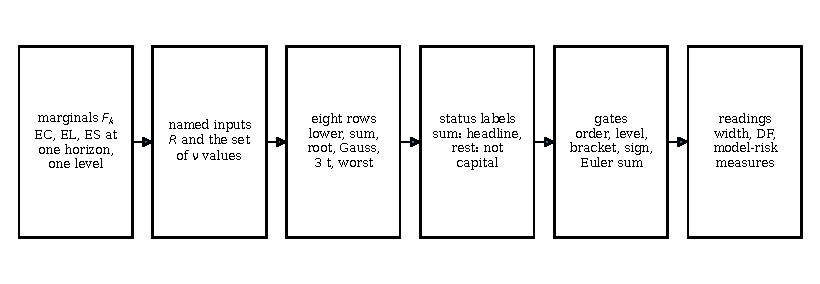
\includegraphics[width=\textwidth]{figures/protocol}
\caption{The flow of the protocol: the marginals at one horizon and one level and the named inputs (a correlation matrix and the set of degrees of freedom) produce the eight rows of the band, each row receives a status label, the checks run on the labelled band, and the readings (width, diversification factors, model-risk measures and the change under the stress) are taken from it.}
\label{fig:protocol}
\end{figure}

\subsection{The rule}
\label{sec:method-rule}

The rule has five clauses. First, an aggregate capital figure is never reported alone: it is reported with the band of aggregation
methods computed on the same marginals. Second, the band has a fixed order and a fixed content: the lower bound, the simple sum,
the square-root rule, the Gaussian copula, one $t$ copula for each degree of freedom of the named set, and the worst case, which for
the set $\{4,8,30\}$ gives eight rows (Table~\ref{tab:protocol}). Third, one horizon and one confidence level apply to every row
and to every marginal. Fourth, exactly one row, the simple sum, carries the status \emph{headline capital}; the seven other rows
carry the status \emph{information, not capital}, and so do the Euler allocation and the model-risk measures. Fifth, the inputs that
are conventions, the correlation matrices and the set of degrees of freedom, are named and labelled as conventions in the same
document, so that a reader sees which part of the band depends on a choice that no data settle.

\begin{table}[htbp]
\centering
\small
\caption{The eight rows of the band in the order in which every aggregate shows them, with the quantity each row reports, how the engine computes it and the status label it carries; only the simple sum is labelled headline capital.}
\label{tab:protocol}
\fitwidth{\begin{tabular}{rp{2.0cm}p{5.2cm}p{2.7cm}p{2.3cm}}
\toprule
\# & Row & Capital of the row & Computation & Status \\
\midrule
\relax 1 & \relax lower bound & \relax best value at risk over all couplings, less the expected losses & \relax rearrangement, outer end of the range & \relax information, not capital \\
\relax 2 & \relax simple sum (headline) & \relax sum of the marginal capitals; the comonotonic row & \relax closed form & \relax headline capital \\
\relax 3 & \relax square-root rule & $\sqrt{\mathrm{EC}^{\top}R\,\mathrm{EC}}$ with the named matrix $R$ & \relax closed form & \relax information, not capital \\
\relax 4 & \relax Gaussian copula & \relax value at risk of the sum under the Gaussian copula of $R$, less expected losses & \relax Monte Carlo, $10^6$ draws & \relax information, not capital \\
\relax 5 & $t$ copula, $\nu=4$ & \relax the same under the $t$ copula with $\nu=4$ and the matrix $R$ & \relax Monte Carlo, $10^6$ draws & \relax information, not capital \\
\relax 6 & $t$ copula, $\nu=8$ & \relax the same with $\nu=8$ & \relax Monte Carlo, $10^6$ draws & \relax information, not capital \\
\relax 7 & $t$ copula, $\nu=30$ & \relax the same with $\nu=30$ & \relax Monte Carlo, $10^6$ draws & \relax information, not capital \\
\relax 8 & \relax worst case & \relax worst value at risk over all couplings, less the expected losses & \relax rearrangement, outer end of the range & \relax information, not capital \\
\bottomrule
\end{tabular}}
\end{table}


The order is not cosmetic. It places the two sharp bounds at the ends and the simple sum next to the lower one, so that the
reader meets the extremes before the diversified figures; it also makes the structure checkable by a program, because a band whose
rows are in another order or whose labels do not follow the method is rejected.

\subsection{The rows of the band}
\label{sec:method-rows}

All rows report a capital on the basis of Equation~\ref{eq:coupling-capital}, the value at risk of the total less the sum of the
expected losses. The simple sum is $H$ of Equation~\ref{eq:ec-headline}. The square-root row combines the marginal capital figures
through the correlation matrix $R$,
\begin{equation}
b_{\mathrm{sqrt}}=\sqrt{\mathrm{EC}^{\top}R\,\mathrm{EC}},
\label{eq:sqrt-row}
\end{equation}
which equals the capital of the total when the losses are jointly elliptical with the matrix $R$ and the same family, and is
otherwise a convention. The copula rows simulate. Let $\xi\sim N(0,I_K)$, let $A$ be the Cholesky factor of $R$ so that $Z=A\xi$
has correlation $R$, and let $W\sim\chi^2_\nu$ be independent of $\xi$. The uniforms of the Gaussian and of the $t$ copula are
\begin{equation}
U_k=\Phi(Z_k),\qquad U_k=t_\nu\!\Big(Z_k\big/\sqrt{W/\nu}\Big),\qquad L_k=Q_k(U_k),
\label{eq:copula-sampling}
\end{equation}
with $\Phi$ the standard normal and $t_\nu$ the Student distribution function. With $S_i=\sum_kL_{ik}$ the total of draw $i$ and $S_{(1)}\le\dots\le S_{(n)}$ its order statistics, the capital of the row and
its Monte Carlo standard error are
\begin{equation}
b=S_{(\lceil n\alpha\rceil)}-\sum_{k=1}^K\mathrm{EL}_k ,\qquad
\mathrm{se}(b)=\frac{1}{\sqrt{B}}\,\mathrm{sd}\big(\widehat q_1,\dots,\widehat q_B\big),
\label{eq:row-capital}
\end{equation}
where $\widehat q_1,\dots,\widehat q_B$ are the sample quantiles at level $\alpha$ of $B=20$ consecutive batches of $n/B$ draws and
$\mathrm{sd}$ is the sample standard deviation. The same seed drives every simulated row, which makes the rows of one band
comparable and the band reproducible.

The two bound rows are not simulated. The lower bound is the smallest value at risk of the total over $\mathcal C$ and the worst
case is the largest, both less $\sum_k\mathrm{EL}_k$, and the rearrangement algorithm of Puccetti and R\"uschendorf
\citep{puccetti2012} computes each as a range. For the upper end, build the two $N\times K$ matrices of quantiles from the upper
tail,
\begin{equation}
\underline x_{ik}=Q_k\!\Big(\alpha+(1-\alpha)\tfrac{i-1}{N}\Big),\qquad
\overline x_{ik}=Q_k\!\Big(\alpha+(1-\alpha)\tfrac{i}{N}\Big),\qquad i=1,\dots,N ,
\label{eq:rearrangement-matrix}
\end{equation}
rearrange each column in turn to be oppositely ordered to the sum of the others, and repeat until the smallest row sum changes
by less than a tolerance $\varepsilon$. The smallest row sums of the two rearranged matrices bracket the worst value at risk
\citep{epr2013}; the lower bound is computed in the same way from the matrices on $[0,\alpha]$ with the largest row sum
minimised. The row reports the outer end of each range, the smallest end for the lower bound and the largest for the worst case,
so that the displayed interval contains the sharp one up to the accuracy of the algorithm.

\subsection{Labels and the headline}
\label{sec:method-labels}

The label of a row is a function of its method and nothing else: the simple sum is \emph{headline capital}, every other method is
\emph{information, not capital}. The functional form matters because it prevents a figure from changing status by being the
smallest, the preferred one or the most recent. A row above the headline is a true result of the method, since the value at risk
is not subadditive (Section~\ref{sec:theory}); the protocol reports it with its diversification factor above one, flags it, and
neither repairs it nor refuses it. The diversification factor $\mathrm{DF}_j=b_j/H$ is reported for every row and is the only
normalisation the band uses. The bank may choose a figure other than the simple sum as its capital, but then the choice is a
decision of the bank and not a label of the protocol, and the label of the headline stays on the simple sum. The label is carried by the document that holds the band, so that it
travels with the figure: a reader who meets a number of the band meets its status beside it. The Euler allocation and the
model-risk measures carry the same status field, and the structure check of Section~\ref{sec:results-structure} fails on a band in which one of these quantities lacks it or
carries a status that does not follow from its method.

\subsection{Allocation and model-risk measures}
\label{sec:method-allocation}

The band is accompanied by two further quantities, both labelled information. The first is the Euler allocation of the aggregate
expected shortfall of a reference copula row, here the Gaussian one. With the sample $S_i=\sum_k L_{ik}$ of $n$ draws, the
Acerbi--Tasche estimator of the expected shortfall and the contribution of risk type $k$ are
\begin{equation}
\widehat{\ES}_\alpha=\frac{1}{1-\alpha}\sum_{i=1}^n w_i S_i ,\qquad
c_k=\frac{1}{1-\alpha}\sum_{i=1}^n w_i L_{ik},\qquad \sum_{k=1}^K c_k=\widehat{\ES}_\alpha ,
\label{eq:euler}
\end{equation}
where $w_i=1/n$ for the draws above the sample quantile, a fractional weight on the draw at the quantile, and zero below
\citep{acerbi2002,tasche2008}. The sum holds by linearity for every sample, so the check on it verifies the implementation and the
bookkeeping of the allocation, not a statistical property of the dependence.

The second quantity is a pair of model-risk measures on the set of models that the band itself supplies. With $\rho_j$ the capital
of row $j$ of the band, $\rho_0$ that of the reference row (the Gaussian copula), $\overline\rho=\max_j\rho_j$ and
$\underline\rho=\min_j\rho_j$, the additive and the relative measure of Barrieu and Scandolo \citep{barrieu2015} are
\begin{equation}
\mathrm{AM}=\frac{\overline\rho}{\rho_0}-1,\qquad \mathrm{RM}=\frac{\overline\rho-\rho_0}{\overline\rho-\underline\rho}\in[0,1].
\label{eq:model-risk}
\end{equation}
$\mathrm{AM}$ is the multiplier that takes the reference figure to the worst figure of the set, and $\mathrm{RM}$ places the
reference between the two ends. The protocol adds the worst case of the expected aggregate loss over reweightings of the
sample within a budget of relative entropy, the measure of Glasserman and Xu \citep{glasserman2014}. All three are sensitivity
information for the validator: none of them is a capital figure.

\subsection{The checks}
\label{sec:method-checks}

The protocol is accompanied by nine tests, each a function that returns a light and the statistic behind it. Their acceptance
criteria are internal to the validation, not regulatory thresholds; a green light means that a statistic fell inside the criterion
and nothing more. Three tests read rows beyond the Gaussian copula. The copula-choice test computes
$\max_{\nu\in\mathcal N}\lvert b_{t,\nu}/b_{\mathrm{G}}-1\rvert$, green up to 0.05, amber up to 0.15 and red above. The bracket
test is red when a row lies outside the interval from the lower bound to the worst case. The correlation-stress test computes the
relative change of the Gaussian row between the base matrix and the stressed matrix, red when it is negative and amber above 0.10.
Six tests read the Gaussian row, the marginals or the conventions. The comparison with the simple sum and the square-root rule
tests whether the aggregate is not above the simple sum and agrees with the square-root rule within 10 percent. The sign test is
red when any diversification factor exceeds one. The consistency test counts the marginals whose horizon or level differs from the
band's and is red when the count is above zero. The additivity test compares the sum of the Euler contributions with the aggregate
expected shortfall. The agreement test compares a Monte Carlo run on elliptical marginals with the square-root row in units of its
standard error, green within three. The reference of Rosenberg and Schuermann compares the additive overestimate of the case with
the published range of 30 to 40 percent and is always green, because it is a reference and not a criterion. The tests make the
rule enforceable: a band with a missing row or a changed label does not pass its checks.

\subsection{Algorithm and complexity}
\label{sec:method-algorithm}

Algorithm~\ref{alg:band} builds the band and Algorithm~\ref{alg:rearrangement} computes the range of the bound rows.

\begin{algorithm}[htbp]
\caption{The dependence band of an aggregate.}
\label{alg:band}
\begin{algorithmic}[1]
\Require quantile functions $Q_1,\dots,Q_K$, expected losses $\mathrm{EL}_k$, capital $\mathrm{EC}_k$, matrix $R$, set $\mathcal N$, level $\alpha$, horizon $h$, draws $n$, seed $s$
\State check that $R$ is a correlation matrix, that every $\nu\in\mathcal N$ exceeds 2 and that $\mathrm{EC}_k\approx Q_k(\alpha)-\mathrm{EL}_k$ for all $k$; otherwise refuse
\State $H\gets\sum_k\mathrm{EC}_k$; $b_{\mathrm{sqrt}}\gets\sqrt{\mathrm{EC}^\top R\,\mathrm{EC}}$
\State $(\underline b,\overline b)\gets$ Algorithm~\ref{alg:rearrangement} on $Q_1,\dots,Q_K$ at level $\alpha$, less $\sum_k\mathrm{EL}_k$
\For{each family in $\{\text{Gaussian}\}\cup\{t_\nu:\nu\in\mathcal N\}$}
\State draw $n$ copula samples with seed $s$ by Equation~\ref{eq:copula-sampling}; $S_i\gets\sum_kQ_k(U_{ik})$
\State $b\gets$ sample $\alpha$-quantile of $S$ less $\sum_k\mathrm{EL}_k$; $\mathrm{se}\gets$ batch-means standard error
\EndFor
\State assemble the rows in the order lower bound, simple sum, square-root, Gaussian, $t_\nu$ for $\nu\in\mathcal N$ ascending, worst case
\State label the simple sum \emph{headline capital} and every other row \emph{information, not capital}; $\mathrm{DF}_j\gets b_j/H$
\State compute the Euler contributions of Equation~\ref{eq:euler} on the Gaussian sample and the measures of Equation~\ref{eq:model-risk}
\State run the nine tests; \Return the band, the labels, the allocation, the measures and the lights
\end{algorithmic}
\end{algorithm}

\begin{algorithm}[htbp]
\caption{Rearrangement range of the worst value at risk (upper end).}
\label{alg:rearrangement}
\begin{algorithmic}[1]
\Require quantile functions $Q_1,\dots,Q_K$, level $\alpha$, cells $N$, tolerance $\varepsilon$, sweep limit $m$, seed $s$
\State build $\underline X$ and $\overline X$ by Equation~\ref{eq:rearrangement-matrix}
\For{$X\in\{\underline X,\overline X\}$}
\State permute each column of $X$ at random under the seed; $v\gets$ smallest row sum of $X$
\Repeat
\For{$k=1$ \textbf{to} $K$}
\State rearrange column $k$ to be oppositely ordered to the sum of the other columns
\EndFor
\State $v'\gets v$; $v\gets$ smallest row sum of $X$
\Until{$\lvert v-v'\rvert<\varepsilon$ \textbf{or} $m$ sweeps}
\State $v_X\gets v$
\EndFor
\State \Return the range $(v_{\underline X},v_{\overline X})$
\end{algorithmic}
\end{algorithm}

One sweep of Algorithm~\ref{alg:rearrangement} sorts $K$ columns of $N$ cells, so it costs $O(KN\log N)$, and the number of sweeps
is small in practice (Section~\ref{sec:results-structure}); the whole bound costs about four times that, one per matrix and end.
Each copula row costs $O(nK^2)$ to draw the correlated normals, $O(nK\log G)$ to evaluate the quantile functions on a grid of
$G$ points and $O(n)$ to select the quantile, and holds $n\times K$ losses in memory, 32 megabytes for the $10^6$ draws and four
risk types of the study. The simple sum and the square-root row cost $O(K^2)$. The allocation sorts the total once, $O(n\log n)$, and the nine tests add a cost that is negligible beside it. On the
committed settings the whole band, with its four simulated rows and its two bound rows, runs in about $\bdBandSeconds$ seconds on one
workstation, of which the rearrangements take about $\bdBoundsSeconds$ seconds; the simulation dominates, and it grows linearly in $n$ while the
standard error of a row falls only as $n^{-1/2}$, which is why the band is not run with more draws than the width of the band
requires.

\subsection{Implementation}
\label{sec:method-implementation}

The protocol is implemented in the engine \texttt{riskvalidation} 1.1.0, module \texttt{aggregation.band}, whose function
\texttt{dependence\_band} returns the whole band and never a scalar. It calls \texttt{aggregation.simple} for the closed-form rows,
\texttt{aggregation.copulas} for the copula rows, \texttt{aggregation.bounds} for the rearrangement, \texttt{portfolio.euler} for
the allocation and \texttt{aggregation.model\_risk} for the measures, and the nine tests are in \texttt{validation.aggregation}
and \texttt{validation.portfolio}. A row object refuses a status that does not follow its method and a degrees-of-freedom value
on a row that is not a $t$ row. The function refuses a marginal capital that does not match its quantile function at the level of
the band, with a tolerance of one percent, so that a marginal read at another level cannot enter the band unnoticed, and it
refuses a correlation matrix that is not a correlation matrix and a set of degrees of freedom that is empty, unsorted or not
above 2. The case uses it with $n=10^6$ draws, the seed 42, a chunk of $10^5$ draws, $N=10^5$ cells and a tolerance
$\varepsilon=10^{-3}$ for the rearrangement. The committed documents of the case hold the band of each aggregate with these
settings, and every experiment of Section~\ref{sec:experimental-design} calls the same function.

\section{Theory}
\label{sec:theory}

This section states what can be proved about the band and what can only be conjectured, with the conditions under which each
statement holds. Throughout, the marginals satisfy the standing assumption of Section~\ref{sec:problem-assumptions}: each $Q_k$ is
continuous and strictly increasing on the region where it is read. The results are labelled [D] when they are derived here or
quoted from the cited source with its proof, and [C] when they are conjectures supported by the experiments.

\subsection{The headline is the comonotonic capital, and the expected shortfall bounds every row}
\label{sec:theory-headline}

\begin{proposition}[Headline and ceiling] [D]
\label{prop:headline}
Let $\pi_{\mathrm{com}}$ be the comonotonic coupling, the law of $(Q_1(U),\dots,Q_K(U))$ for one uniform variable $U$. Then
\begin{equation}
b(\pi_{\mathrm{com}})=H=\sum_k\mathrm{EC}_k .
\label{eq:comonotonic}
\end{equation}
For every coupling $\pi\in\mathcal C$,
\begin{equation}
b(\pi)\le\sum_{k=1}^K\ES_\alpha(L_k)-\sum_{k=1}^K\mathrm{EL}_k ,
\label{eq:es-ceiling}
\end{equation}
and the value at risk of the total can exceed $\sum_k\VaR_\alpha(L_k)$, so that $\overline b>H$ is possible.
\end{proposition}

\begin{proof}
Under $\pi_{\mathrm{com}}$ the total is $S=g(U)$ with $g=\sum_kQ_k$, which is continuous and strictly increasing by the standing
assumption. Then $\Prob(S\le x)=g^{-1}(x)$ on the range of $g$, so $\VaR_\alpha(S)=g(\alpha)=\sum_kQ_k(\alpha)=\sum_k\VaR_\alpha(L_k)$.
Subtracting $\sum_k\mathrm{EL}_k$ gives Equation~\ref{eq:comonotonic}. For Equation~\ref{eq:es-ceiling}, the expected shortfall
is the mean of the quantiles above $\alpha$, each at least $Q_S(\alpha)$, so $\VaR_\alpha(S_\pi)\le\ES_\alpha(S_\pi)$; the expected
shortfall is subadditive \citep{acerbi2002,artzner1999}, so $\ES_\alpha(S_\pi)\le\sum_k\ES_\alpha(L_k)$. The last claim is not a
consequence of the first two: the value at risk is not subadditive, and the sharp worst case of Section~\ref{sec:results-band} is
an instance with $\overline b>H$ \citep{ems2002,epr2013}.
\end{proof}

The proposition says two things about the band. The simple sum is not an arbitrary figure: it is the capital of the one coupling
in which the risk types reach their quantiles together. And the simple sum is not a ceiling either, since a coupling that is not
comonotonic can put more of the loss above the quantile. The ceiling that does hold is the sum of the expected shortfalls, which
for Banco Andino is CLP \bdSumEs{} billion of value at risk against the worst case of CLP \bdWorstVar{} billion, a slack of
CLP \bdSlack{} billion that the numerical bound must respect (Section~\ref{sec:results-structure}).

\subsection{Bracketing and invariance of the bounds}
\label{sec:theory-bracket}

\begin{proposition}[Bracket and invariance] [D]
\label{prop:bracket}
For every coupling $\pi\in\mathcal C$, $\underline b\le b(\pi)\le\overline b$. In particular every row of the band that is the
capital of a coupling lies in $[\underline b,\overline b]$: the simple sum, the Gaussian copula row and each $t$ copula row. The
numbers $\underline b$ and $\overline b$ are functions of $(Q_1,\dots,Q_K,\alpha)$ and of $\sum_k\mathrm{EL}_k$ only, so they do
not change with the correlation matrix, with the degrees of freedom or with any other dependence input.
\end{proposition}

\begin{proof}
The first claim is the definition of the infimum and the supremum in Equation~\ref{eq:sharp-bounds}. The rows named are capitals of
couplings: $\pi_{\mathrm{com}}$ by Proposition~\ref{prop:headline}, and the Gaussian and $t$ copulas with the marginals $Q_k$ by
Equation~\ref{eq:copula-sampling}. The set $\mathcal C$ and the functional $\VaR_\alpha(S_\pi)$ are defined from the marginals and
the level alone, so the bounds cannot depend on $R$ or $\nu$.
\end{proof}

Two limits belong to the statement. The square-root row of Equation~\ref{eq:sqrt-row} is not in general the capital of a coupling,
so Proposition~\ref{prop:bracket} does not place it in the interval, and the bracket test exists to check that it falls inside.
And the rearrangement algorithm that computes the bounds has no proof of convergence for all initial configurations: its authors
state a proof of convergence as an open problem \citep{puccetti2012,hofert2015}. The evidence that the algorithm has converged on
the marginals of the study is empirical: four independent runs end in ranges whose widths are
CLP \bdLowerRangeWidth{} billion for the lower bound and CLP \bdUpperRangeWidth{} million for the worst case
(Section~\ref{sec:results-structure}). Figure~\ref{fig:rearrangement} shows what the algorithm does to the tail of the study.

\begin{figure}[htbp]
\centering
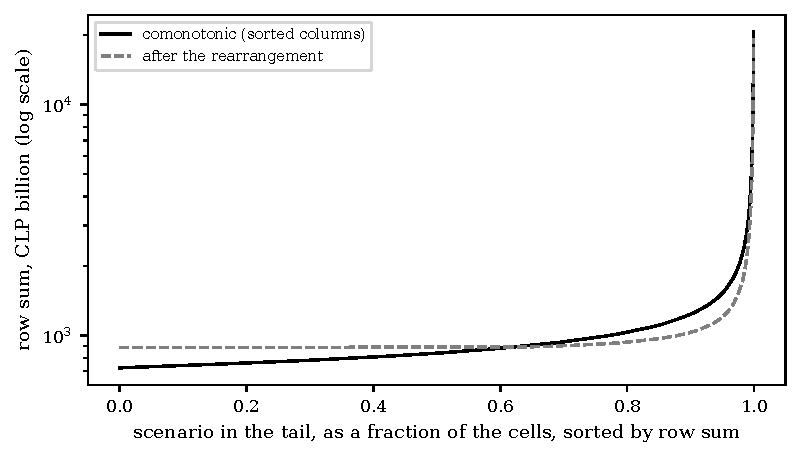
\includegraphics[width=0.78\textwidth]{figures/rearrangement}
\caption{The row sums of the $\bdRearrCells$ upper-tail cells of the four marginals of Banco Andino, in CLP billion on a logarithmic scale and sorted: with the columns sorted alike (comonotonic, solid line) and after the rearrangement of each column against the sum of the others (dash-dotted line). The smallest row sum rises from CLP \bdRearrMinComo{} to \bdRearrMinAfter{} billion, the worst value at risk, because the large losses of one risk type are moved to the cells where the others are small.}
\label{fig:rearrangement}
\end{figure}

\subsection{Dependence that the matrix does not carry}
\label{sec:theory-tails}

\begin{proposition}[Same rank correlation, different tails] [D]
\label{prop:tails}
Let $C^{\mathrm G}_R$ and $C^{t}_{R,\nu}$ be the Gaussian copula and the $t$ copula with the same correlation matrix $R$. Kendall's
rank correlation of the pair $(i,j)$ is the same for both,
\begin{equation}
\tau_{ij}=\frac{2}{\pi}\arcsin\rho_{ij},
\label{eq:kendall}
\end{equation}
and their upper tail dependence coefficients differ: for $\lvert\rho\rvert<1$ the Gaussian coefficient is zero, while the $t$
coefficient is
\begin{equation}
\lambda_\nu(\rho)=2\,t_{\nu+1}\!\left(-\sqrt{\frac{(\nu+1)(1-\rho)}{1+\rho}}\right)>0 ,
\label{eq:tail-dependence}
\end{equation}
which tends to zero as $\nu\to\infty$.
\end{proposition}

\begin{proof}
Equation~\ref{eq:kendall} holds for every elliptical distribution with continuous margins \citep{lindskog2003}. The tail
dependence coefficients of the Gaussian and the $t$ copulas are derived in \citet{demarta2005} and \citet{ems2002}: the
Gaussian coefficient vanishes for $\rho<1$ because the conditional law of one standardised variable given a large value of the
other is centred at $\rho$ times that value, and the $t$ coefficient follows from the same conditioning with the
$t_{\nu+1}$ law of the standardised residual. As $\nu\to\infty$ the argument of $t_{\nu+1}$ in Equation~\ref{eq:tail-dependence}
tends to $-\infty$ at the rate $\sqrt\nu$ and the coefficient to zero.
\end{proof}

At the pair correlation $\rho=0.5$ of the base matrix the coefficient is $\bdTLambdaFour$ for $\nu=4$ and $\bdTLambdaThirty$ for
$\nu=30$, and at $\rho=0.2$ it is $\bdTLambdaLowFour$ for $\nu=4$. The consequence for the band is that the three $t$ rows and
the Gaussian row share one matrix and one rank correlation and differ only in the tail dependence at the level where the capital
is read. That is why a correlation matrix alone cannot report the dependence uncertainty of the aggregate, and why the band holds
several degrees of freedom and not one.

\begin{remark}[Monotone in the degrees of freedom] [C]
\label{conj:nu}
For positively correlated risks with the marginals of the study, the capital of the $t$ copula row decreases as $\nu$ increases
and approaches the Gaussian row. The mechanism is the decrease of $\lambda_\nu(\rho)$ with $\nu$. The evidence is the curve of
Figure~\ref{fig:nu-curve} for the base and for the stressed matrix over eight values from 2.5 to 100: the capital is non-increasing
in $\nu$ up to two combined standard errors on both matrices, and at $\nu=100$ it exceeds the Gaussian row by CLP \bdNuHundredGap{}
billion, within the Monte Carlo error. It is a conjecture because the dependence of a quantile of a sum on $\nu$ can be non-monotone
for marginals with another shape of tail, and no proof is offered for the marginals of the study.
\end{remark}

\subsection{Closed forms for the square-root row and the allocation}
\label{sec:theory-closed}

\begin{proposition}[Shift of the square-root row] [D]
\label{prop:sqrt}
Let $\mathrm{EC}\ge0$ and let $R'$ differ from $R$ only in the pair $(i,j)$, where $\rho_{ij}'=\rho_{ij}+\Delta$. Then
\begin{equation}
b_{\mathrm{sqrt}}(R')^2-b_{\mathrm{sqrt}}(R)^2=2\Delta\,\mathrm{EC}_i\,\mathrm{EC}_j .
\label{eq:sqrt-shift}
\end{equation}
If every entry of $R$ lies in $[0,1]$, then $\sqrt{\sum_k\mathrm{EC}_k^2}\le b_{\mathrm{sqrt}}\le H$.
\end{proposition}

\begin{proof}
Write $\mathrm{EC}^\top R\,\mathrm{EC}=\sum_k\mathrm{EC}_k^2+2\sum_{k<l}\rho_{kl}\mathrm{EC}_k\mathrm{EC}_l$ and take the difference
for the two matrices, in which only the term $(i,j)$ changes. For the bounds, replace every off-diagonal entry by 0 for the lower
bound and by 1 for the upper bound, using $\mathrm{EC}\ge0$; the upper bound is $\sqrt{(\sum_k\mathrm{EC}_k)^2}=H$.
\end{proof}

For Banco Andino the stress that raises the market-credit correlation from 0.5 to 0.8 gives, by Equation~\ref{eq:sqrt-shift},
a change of $2\cdot0.3\cdot\mathrm{EC}_{\mathrm{credit}}\mathrm{EC}_{\mathrm{market}}=\bdVcClosedDiff\times10^{9}$ in CLP million
squared, and the committed rows give $\bdVcSquareDiff\times10^{9}$: the identity is met by the committed documents to the digits
shown. The floor of the proposition is CLP \bdSqrtFloor{} billion and the ceiling is the headline of CLP \bdHeadline{} billion;
the square-root row of CLP \bdVc{} billion lies between them.

\begin{proposition}[Additivity of the allocation] [D]
\label{prop:euler}
With the weights of Equation~\ref{eq:euler}, $\sum_kc_k=\widehat{\ES}_\alpha$ for every sample. If $\ES_\alpha$ is
differentiable in the weights, the contribution $c_k$ is its derivative with respect to the weight of risk type $k$ at the unit
weights.
\end{proposition}

\begin{proof}
For each draw $\sum_kL_{ik}=S_i$, so $\sum_kc_k=(1-\alpha)^{-1}\sum_iw_iS_i=\widehat{\ES}_\alpha$. The expected shortfall of
$\sum_kw_kL_k$ is positively homogeneous of degree one in $w$, so Euler's theorem on homogeneous functions gives
$\sum_kw_k\,\partial\ES_\alpha/\partial w_k=\ES_\alpha$; the identification of the derivative with the conditional expectation of
$L_k$ given the tail event is the Euler principle \citep{tasche2008}.
\end{proof}

The additivity is therefore an identity of the estimator, and a test of it checks the implementation. What is not an identity
is the allocation itself, which carries the sampling error of the tail of the sample: the shares in Table~\ref{tab:euler} have a
standard deviation of about one percentage point over independent seeds.

\subsection{Sampling error, and what coverage by the sharp range means}
\label{sec:theory-sampling}

The simulated rows are sample quantiles at $\alpha=0.999$, which rest on the $n(1-\alpha)$ largest draws, 1,000 of the $10^6$.
For independent draws the standard error of the sample quantile of the total is, asymptotically,
\begin{equation}
\mathrm{se}(\widehat q_\alpha)\approx\frac{\sqrt{\alpha(1-\alpha)/n}}{f_S(q_\alpha)} ,
\label{eq:quantile-se}
\end{equation}
with $f_S$ the density of the total \citep{glasserman2003}; the engine estimates it by batch means, without the density. The
error is below one percent of a row ($\bdGaussSd$ CLP billion on the Gaussian row over independent seeds)
and it is two orders of magnitude below the width of the band, which is the reason the rows can be compared (Section~\ref{sec:results-band}).

\begin{proposition}[Coverage by the sharp range] [D]
\label{prop:coverage}
Let $\pi^\ast\in\mathcal C$ be any planted dependence structure with the marginals $Q_k$. Then $b(\pi^\ast)\in[\underline b,\overline b]$.
\end{proposition}

\begin{proof}
It is the first claim of Proposition~\ref{prop:bracket} applied to $\pi^\ast$.
\end{proof}

The proposition has a consequence for the design. The coverage of the planted structures by the sharp range cannot be an
empirical finding about the structures: it holds for every structure, up to the error of the three estimated quantities, the
capital of the structure and the two ends of the range. The experiment that measures it is a verification of the implementation
against the theory, and its empirical content is the width of the interval, that is, how much of the interval is slack for the
structures that a bank might plausibly face. The interior rows are different. The interval spanned by the five interior rows is the
range of the capitals of five specific couplings, and whether it contains the capital of another coupling is an empirical question
that depends on the coupling: Proposition~\ref{prop:tails} says that a structure whose tail dependence or whose matrix lies outside
what the five rows span can fall outside. Section~\ref{sec:results-planted} measures it.

\section{Experimental design}
\label{sec:experimental-design}

The experiments test whether the protocol does what Section~\ref{sec:method-rule} says, how much of the dependence uncertainty
the band spans, and what each component contributes. They run the engine on the committed documents of the case and on planted
dependence structures whose capital is known by simulation. Every number in Section~\ref{sec:results} comes from a script that
is committed beside the manuscript and is run from the repository root.

\subsection{The predictions}
\label{sec:design-hypotheses}

The nine predictions were set by the author for this study; the design record of the protocol states no acceptance criteria, so they
were not taken from a prior specification. They are written to \texttt{experiments/hypotheses.json}, which the experiment scripts
read. By file time they were written on 6 November 2026, before the runs of the reproduction, planted-structure and ablation
experiments (H2 to H4c, H6 and H7). Their order relative to the first run of the structure experiment (H1 and H5) is not recorded,
and the file was first versioned together with the results. Each prediction is stated with the outcome that refutes it.
\begin{description}
\item[H1, structure.] In each of the six committed aggregates the band has eight rows in the stated order, exactly one row labelled
headline capital and it is the simple sum, seven rows labelled information, one horizon and one confidence level, and an Euler
allocation that adds up to the aggregate expected shortfall to a relative error of at most $10^{-6}$. Refuted if any aggregate fails
any element.
\item[H2, reproduction.] The engine, given the marginals rebuilt from the committed quantile grids and the committed seed, returns
every row of the committed band within the larger of three combined Monte Carlo standard errors and 0.5 percent of the committed
row. Refuted if any row differs by more.
\item[H3, the band is not noise and no row speaks for it.] The width of the band, the worst case less the lower bound, is at least
100 times the largest Monte Carlo standard error of its rows, and for every row some other row differs from it by more than 10
percent. Refuted if the width is below 100 standard errors or some row lies within 10 percent of every other row.
\item[H4a, coverage by the sharp range.] Over the planted structures the interval from the lower bound to the worst case contains
the capital of the structure in all of them, after widening it by three standard errors of the capital of the structure.
\item[H4b, coverage by the interior rows.] The interval spanned by the five interior rows of the band (the square-root rule, the Gaussian copula
and the $t$ copulas with 4, 8 and 30 degrees of freedom) contains the capital of the structure in at least 75 percent of the
structures. Refuted if fewer are covered. ``The band'' here is the base band, computed with the base matrix, which is the stricter
reading; Section~\ref{sec:results-planted} also reports the reading with the interior rows of both matrices, so the refutation does
not depend on the reading.
\item[H4c, a single figure is not reliable.] The Gaussian copula row alone lies within 5 percent of the capital of the structure in
at most half of the structures. Refuted if more than half are within 5 percent.
\item[H5, invariance of the bounds.] The lower bound and the worst case are equal in the base band and in the band under the
market-credit correlation of 0.8 (relative difference below $10^{-9}$), while the Gaussian copula row moves by more than 10
percent.
\item[H6, the common horizon and level matter.] Reading one marginal, the market marginal, at 99 percent in place of 99.9 percent
changes the simple sum by at least 10 percent, and the consistency test returns red on that band.
\item[H7, each row feeds a test.] Removing the $t$ rows leaves the copula-choice test unrunnable and removing the stressed band
leaves the correlation-stress test unrunnable; with the Gaussian row alone, at most half of the nine tests can be run.
\end{description}
H4a is a consequence of Proposition~\ref{prop:coverage}; its outcome verifies the implementation and carries no information about
the structures.

\subsection{Data and provenance}
\label{sec:design-data}

The data are the committed documents of case C18 of Contraste, the aggregation of capital under macroeconomic scenarios, for
Banco Andino. The bank is synthetic and its loss models are simulated, so no statement below is about the capital of any
actual bank. There are four scenario documents, the baseline, the adverse scenario of the European Banking Authority 2025, the
severely adverse scenario of the Federal Reserve 2026 and the delayed-transition scenario of the Network for Greening the
Financial System, and a fifth document, the $t$ copula variant of the baseline, which also holds the band under the
market-credit correlation of 0.8. The five documents carry one and the same aggregation block, shown by its SHA-256 digest, and
the block of the stress is the sixth aggregate: the six aggregates reduce to $\bdDistinct$ distinct ones. The marginals come from four producers: the credit marginal from the engine's
grouped copula on six portfolio segments with 400 representative names each, the market marginal from the committed mixed-portfolio
forecast of the market case moved from 99 percent and one day to 99.9 percent and one year by the normal quantile ratio and the
square root of 250, the interest rate marginal from the engine's one-factor Hull--White simulation on the curve and the book of
the interest-rate case, and the operational marginal from the Fourier aggregation of a Poisson--generalised Pareto compound
whose parameters are those of the operational-risk case scaled by assets.

The documents commit the expected loss, the value at risk, the expected shortfall and the capital of each marginal and, for each
marginal, its quantile function on a grid of $\bdGridPoints$ probabilities, the standard normal distribution function at the points from
$-4.9$ to $4.9$ in steps of $0.005$, which reaches probabilities of $5\times10^{-7}$ at each end; the simulated samples are not
committed. The experiments rebuild each marginal by linear interpolation of the committed grid, which is the same rule that
produced the committed band, and the quantile function is clamped at the ends of the grid. The market marginal has losses below
zero, a market gain, down to CLP \bdMarketGridMin{} billion at the lower end of its grid. Table~\ref{tab:marginals} gives the
four marginals.

\subsection{Planted dependence structures}
\label{sec:design-planted}

To know what the band contains, the capital of the aggregate must be known under a dependence structure that is not read from the
band. Ten structures are planted on the four marginals of Banco Andino. Four are Gaussian copulas: with the base matrix, with
the matrix of the market-credit stress, with a crisis matrix in which the three financial risks have a correlation of 0.8 with
each other and 0.4 with operational risk, and with independent risks. Three are $t$ copulas: with 3 degrees of freedom and the
base matrix, with 2.5 degrees of freedom and the base matrix, and with 3 degrees of freedom and the crisis matrix; the degrees
of freedom are below the set of the band. One is a mixture of two Gaussian regimes in which 5 percent of the draws come from the
crisis matrix and the others from the base matrix. Two are copulas of families that are not in the band: a reflected Clayton copula,
which has upper tail dependence as a loss tail needs, with the parameter $\theta=\bdClaytonTheta$ that gives the mean Kendall rank
correlation $\bar\tau=\bdTauBar$ of the base matrix, and a Gumbel copula with $\theta=\bdGumbelTheta$ and the same mean. The Clayton and Gumbel
samplers are written for this study, because the engine does not simulate them, and each is checked against its closed
form: the Laplace transform of the stable variable used by the Gumbel sampler, and the rank correlation of each copula
(simulated $\bdClaytonTauSim$ against $\bdClaytonTauExact$ for the Clayton copula at $\theta=2$, and $\bdGumbelTauSim$ against
$\bdGumbelTauExact$ for the Gumbel copula at $\theta=1.67$; the difference of 0.006 for the Gumbel check is twice the standard
error of Kendall's coefficient on 50,000 pairs). The ten structures are the choice of the author: they span matrices, degrees of
freedom and families inside and outside the band, and they are not a sample from a population of dependence structures of banks.

\subsection{Methods compared}
\label{sec:design-methods}

Every method is run by the product on the same marginals, and none is taken from its publication. The rows of the band are the
simple sum, the square-root rule, the Gaussian copula \citep{li2000,rosenberg2006}, the $t$ copula \citep{demarta2005} at
4, 8 and 30 degrees of freedom, and the sharp bounds by the rearrangement algorithm \citep{puccetti2012,epr2013}. Two further
methods are single-figure estimators that a bank could use in place of the band, given the most favourable input: data from the
planted structure itself. The hybrid value at risk of Rosenberg and Schuermann \citep{rosenberg2006} combines the quantile of each
marginal with the empirical Pearson correlation of a sample of the structure, $\sqrt{v^\top R_{\mathrm{emp}}v}$ with $v_k$ the
sample quantile of marginal $k$, less the expected losses. The calibrated Gaussian copula takes the rank correlation of a sample of
the structure, converts it to a correlation by $\rho=\sin(\pi\tau/2)$, the inverse of Equation~\ref{eq:kendall}, and simulates the
Gaussian copula with that matrix. Both are calibrated on a sample of 200,000 draws of the structure (the rank correlation on its first 50,000), kept apart from
the draws that define its capital. They represent a bank that observes the joint tail with a long sample and which can estimate a matrix perfectly, so
their errors are expected to be smaller than those of a bank.

\subsection{Metrics}
\label{sec:design-metrics}

For a planted structure $s$ the capital $b^\ast(s)$ is the mean of $R_s=20$ independent estimates of Equation~\ref{eq:coupling-capital}
on $10^6$ draws each, with the standard error $\mathrm{se}^\ast(s)=\mathrm{sd}/\sqrt{R_s}$. The error of a single figure $b_j$ is
\begin{equation}
e_j(s)=\frac{b_j}{b^\ast(s)}-1 ,
\label{eq:relative-error}
\end{equation}
and a figure is within the tolerance $\delta$ of the structure when $\lvert e_j(s)\rvert\le\delta$, with $\delta=0.05$ unless
stated. An interval $[\ell,u]$ covers the structure when, after widening by three standard errors of the capital of the structure,
\begin{equation}
\ell-3\,\mathrm{se}^\ast(s)\le b^\ast(s)\le u+3\,\mathrm{se}^\ast(s),
\label{eq:coverage-indicator}
\end{equation}
and the coverage of a set of $M$ structures is the share of those covered. The width of an interval relative to the capital is
$(u-\ell)/b^\ast(s)$; it is the price of coverage, because an interval that is wide enough covers everything. The reproduction of
a committed row uses the combined standard error $\sqrt{\mathrm{se}_{\mathrm{rebuilt}}^2+\mathrm{se}_{\mathrm{committed}}^2}$, and the
width of the band in standard errors is $(b_{\mathrm{worst}}-b_{\mathrm{lower}})/\max_j\mathrm{se}_j$, the maximum taken over the
simulated rows. The difference between the rows is measured by the largest relative difference from a row to another row,
$\max_{l\ne j}\lvert b_l/b_j-1\rvert$. The relative error is signed, so that an underestimate, the dangerous direction for a
capital figure, is told apart from an overestimate, and the median and the maximum of its absolute value summarise it over the
structures. The widening by three standard errors is a common convention that makes the indicator insensitive to the
estimation error of the capital of the structure; it favours an interval by less than the tolerance of 5 percent, since the
standard error of every capital is under one percent of it.

\subsection{Repetitions, seeds and statistics}
\label{sec:design-statistics}

The committed band was produced with the seed 42, $10^6$ draws and $10^5$ cells for the bounds, and the reproduction (H2) runs the
engine at that seed. The variation of the band over the seed is measured by 20 independent runs of the base band (seeds 1001 to
1020) and 10 of the stressed band (seeds 2001 to 2010), reported as the mean and the standard deviation over runs. The capital of
planted structure number $s$, counted from 0, uses the seeds $3001+100s+r$ for $r=0,\dots,19$, its calibration sample the seed
$9001+s$, and the calibrated Gaussian copula the seed $9501+s$. The Euler allocation is repeated over the 20 seeds 4001 to 4020. The
tests of H1, H5, H6 and H7 are deterministic functions of the committed documents and of the engine, and have no repetitions. The
interval of every uncertainty is the standard deviation over seeds, or three standard errors where an interval is widened. No
hypothesis test with a $p$-value is used: each prediction is a stated threshold on a measured quantity, and the table of outcomes
reports the measured value beside the threshold.

\subsection{Ablations planned}
\label{sec:design-ablation}

Four components of the protocol are removed one at a time and the loss is measured on the planted structures. The sharp bounds are
removed, leaving the five interior rows of both matrices. The stressed matrix is removed, leaving the interior rows of the base
matrix. The $t$ rows are removed, leaving the square-root rule and the Gaussian row. And each row is used alone, as a single figure,
with its coverage at the tolerance of 5 percent. The component that is not an interval, the common horizon and level, is ablated
by reading one marginal at another level (H6), and the checks are ablated by removing the rows each reads (H7). The Euler
allocation is compared with the allocation by stand-alone expected shortfall, which does not add up. Each ablation is evaluated on
the same ten structures and the same rows, so that the variants differ only in the component removed and the capital of the
structures is not re-estimated; the interval ends are the means of the independent runs of the band, so that they do not carry
the sampling error of a single run.

\section{Results}
\label{sec:results}

The results follow the order of the predictions. Money is in CLP billion. A $\pm$ interval is a standard deviation over
independent seeds unless a caption says otherwise. Table~\ref{tab:hypotheses}, at the end of the section, lists every prediction
with its measured value and whether it held.

\subsection{Structure of the committed aggregates}
\label{sec:results-structure}

All $\bdAggregates$ committed aggregates satisfy the structure of the rule (H1). Each has eight rows in the order of
Table~\ref{tab:protocol}, one row labelled headline capital and it is the simple sum, seven rows labelled information, one horizon
of one year and one level of 0.999, an Euler allocation and model-risk measures labelled information, and an Euler allocation
whose sum differs from the aggregate expected shortfall by a relative $\bdEulerGap$. The six aggregates reduce to $\bdDistinct$
distinct ones: the five documents carry one aggregation block, and the market-credit stress is the other. The simple sum and the
square-root row, recomputed by the engine from the committed marginal capital and the committed matrix, equal the committed rows
to a relative $10^{-12}$.

The two bound rows converge. The four rearrangements behind them ran $\bdSweeps$ sweeps, the range of the lower bound is CLP
\bdLowerRangeLo{} to \bdLowerRangeHi{} billion of value at risk, a width of \bdLowerRangeWidth{} billion, and the range of the
worst case is CLP \bdUpperRangeLo{} to \bdUpperRangeHi{} billion, a width of \bdUpperRangeWidth{} million. The worst value at risk
of CLP \bdWorstVar{} billion is below the ceiling of Proposition~\ref{prop:headline}, the sum of the expected shortfalls of the
marginals, CLP \bdSumEs{} billion, by CLP \bdSlack{} billion, and the comonotonic value at risk is CLP \bdComoVar{} billion: the
worst case is $\bdWorstOverEs$ of the ceiling and exceeds the comonotonic value, as the proposition allows. On the committed
aggregate the nine tests return green for seven and amber for two: the copula-choice statistic is $\bdCopulaStat$ percent, between
the green limit of 5 and the red limit of 15, and the correlation-stress statistic is $\bdStressStat$ percent, above the amber limit
of 10. The reference of Rosenberg and Schuermann reports an additive overestimate of $\bdRsOver$ percent for the case, inside their
published range of 30 to 40 percent.

\subsection{The band of Banco Andino}
\label{sec:results-band}

Table~\ref{tab:main-results} and Figure~\ref{fig:band} give the band. The headline is CLP \bdHeadline{} billion. The lower bound is
CLP \bdLower{} billion, a diversification factor of \bdLowerDf, and the worst case is CLP \bdWorst{} billion, a factor of \bdWorstDf{},
so the worst case lies $\bdWorstAbove$ percent above the headline. The band is CLP \bdWidth{} billion wide, $\bdWidthOverHeadline$ times
the headline. The interior rows fall between CLP \bdGauss{} billion for the Gaussian copula and CLP \bdTFour{} billion for the $t$
copula with 4 degrees of freedom; the Gaussian row is $\bdGaussBelow$ percent below the headline, which is the same fact as the
simple sum exceeding it by $\bdAdditiveOver$ percent.

\begin{table}[htbp]
\centering
\small
\caption{The dependence band of Banco Andino at one year and 99.9 percent in CLP billion: the committed rows with their Monte Carlo standard error and diversification factor against the simple sum, then the rows rebuilt by the engine from the committed marginal grids as mean and standard deviation over independent seeds (20 for the base matrix, 10 for the matrix with market-credit correlation 0.8) and the relative change under the stress. The two bound rows do not move with the matrix.}
\label{tab:main-results}
\fitwidth{\begin{tabular}{lrrrrr}
\toprule
Row & Committed & DF & Rebuilt, base & Rebuilt, market-credit 0.8 & Change \\
\midrule
\relax lower bound & \relax 118.5 & \relax 0.180 & \relax 118.5 $\pm$ 0.0 & \relax 118.5 $\pm$ 0.0 & \relax +0.000 \\
\relax simple sum (headline) & \relax 658.0 & \relax 1.000 & \relax 658.0 $\pm$ 0.0 & \relax 658.0 $\pm$ 0.0 & \relax +0.000 \\
\relax square-root rule & \relax 528.1 & \relax 0.803 & \relax 528.1 $\pm$ 0.0 & \relax 568.5 $\pm$ 0.0 & \relax +0.077 \\
\relax Gaussian copula & \relax 492.0 $\pm$ 2.5 & \relax 0.748 & \relax 488.1 $\pm$ 3.2 & \relax 549.7 $\pm$ 2.5 & \relax +0.126 \\
$t$ copula, $\nu=4$ & \relax 552.4 $\pm$ 3.4 & \relax 0.839 & \relax 546.9 $\pm$ 4.1 & \relax 584.4 $\pm$ 3.0 & \relax +0.068 \\
$t$ copula, $\nu=8$ & \relax 528.3 $\pm$ 2.8 & \relax 0.803 & \relax 522.7 $\pm$ 3.7 & \relax 572.4 $\pm$ 3.3 & \relax +0.095 \\
$t$ copula, $\nu=30$ & \relax 499.1 $\pm$ 3.3 & \relax 0.759 & \relax 498.8 $\pm$ 3.1 & \relax 558.3 $\pm$ 4.5 & \relax +0.119 \\
\relax worst case & \relax 823.3 & \relax 1.251 & \relax 823.3 $\pm$ 0.0 & \relax 823.3 $\pm$ 0.0 & \relax 0.000 \\
\bottomrule
\end{tabular}}
\end{table}


\begin{figure}[htbp]
\centering
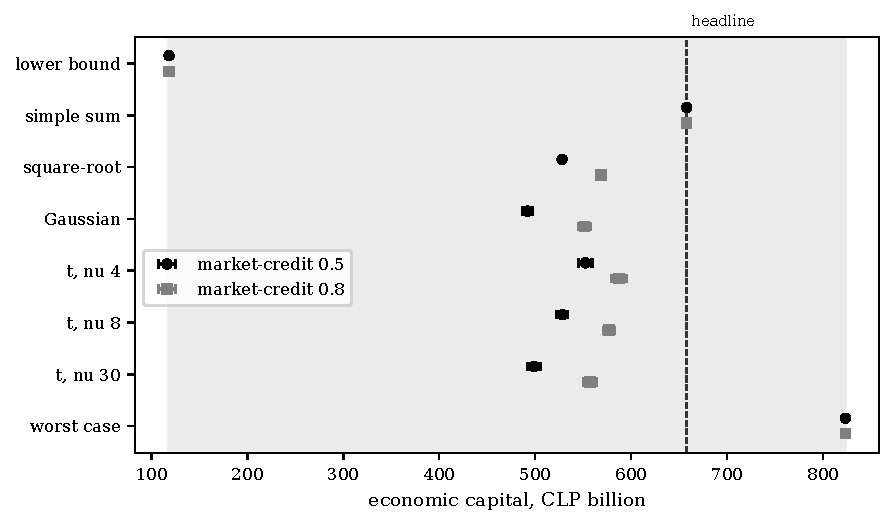
\includegraphics[width=0.86\textwidth]{figures/band}
\caption{The band of Banco Andino at one year and 99.9 percent: the capital of each row in CLP billion for the base matrix (circles) and for the matrix with market-credit correlation 0.8 (squares), with two standard errors where the row is simulated, the interval from the lower bound to the worst case shaded and the headline marked by the dashed line.}
\label{fig:band}
\end{figure}

\emph{Reproduction (H2).} The engine, run on the marginals rebuilt from the committed quantile grids with the committed seed,
returns every committed row to within \bdMaxRelDiff{} percent: the closed-form rows exactly, the lower bound to \bdLowerRelDiff{}
percent and the worst case to \bdWorstRelDiff{} percent (the random start of the rearrangement), and the Gaussian row to
\bdGaussRelDiff{} percent. Each difference is below the tolerance of three combined standard errors or half a percent. The
committed documents are therefore reproduced from the committed marginal grids alone, which is the property that lets a reader
check the band without the simulated samples. The $\bdRepsBase$ independent runs of Table~\ref{tab:main-results} show the sampling
variation: the standard deviation is CLP \bdGaussSd{} billion for the Gaussian row, CLP \bdTFourSd{} billion for the $t$ row with 4
degrees of freedom and at most CLP \bdMaxSd{} billion for any row, and $\bdBoundsSd$ billion for the bound rows.

\emph{The band is not noise (H3).} The width of CLP \bdWidth{} billion is \bdWidthOverSe{} times the largest Monte Carlo standard
error, CLP \bdMaxSe{} billion, which is above the 100 that the prediction required. No row speaks for the band: the largest relative difference from a row to another row is
$\bdFarthestMin$ percent for the Gaussian copula, the row with the smallest such difference, and rises to $\bdFarthestMax$ percent
for the lower bound. No single row is within three quarters of every other.

\emph{Invariance of the bounds (H5).} The stress that raises the market-credit correlation to 0.8 leaves the lower bound and the
worst case unchanged to the precision of the documents, as Proposition~\ref{prop:bracket} requires, while the Gaussian row moves by
$\bdGaussMove$ percent in the committed documents (the rebuilt means in Table~\ref{tab:main-results} show $+0.126$): above the 10
percent of the prediction. The $t$ rows move less, by $\bdTFourMove$ percent for 4 degrees of freedom, $\bdTEightMove$ percent
for 8 and $\bdTThirtyMove$ percent for 30, and the square-root row by $\bdVcMove$ percent. The ordering is that of the tail
dependence: the stress adds least where the $t$ copula already has the most tail dependence, and most where the copula has
almost none. After the stress the interior rows, CLP \bdGaussStress{} to \bdTFourStress{} billion, are still below the headline.

\subsection{The \texorpdfstring{$t$}{t} row as a function of the degrees of freedom}
\label{sec:results-nu}

Figure~\ref{fig:nu-curve} gives the capital of the $t$ copula row for eight values of $\nu$ and the two matrices. On the base
matrix it falls from CLP \bdTTwoFive{} billion at $\nu=2.5$ and \bdTThree{} at $\nu=3$ to \bdTHundred{} at $\nu=100$, a span of
CLP \bdNuSpanBase{} billion or $\bdNuSpanPc$ percent of the smallest value, and the curve approaches the Gaussian row, CLP \bdGauss{}
billion at the committed seed. The three values of the set, 4, 8 and 30, give CLP \bdTFour{}, \bdTEight{} and \bdTThirty{} billion at the committed seed, the last
within $\bdCopulaDiffThirty$ percent of the Gaussian row, so the set spans the curve from the heavy tail to the nearly Gaussian one;
the values below 4 are outside the set and lie within the noise of the value at 3.
The curve is monotone within two combined standard errors on both matrices, the evidence for the conjecture of
Section~\ref{sec:theory-tails}, and the segment from $\nu=2.5$ to $3$ is flat within the noise. The tail dependence coefficient at the pair
correlation of 0.5 falls over the same range from $\bdTLambdaTwoFive$ at $\nu=2.5$ to $\bdTLambdaThirty$ at $\nu=30$.

\begin{figure}[htbp]
\centering
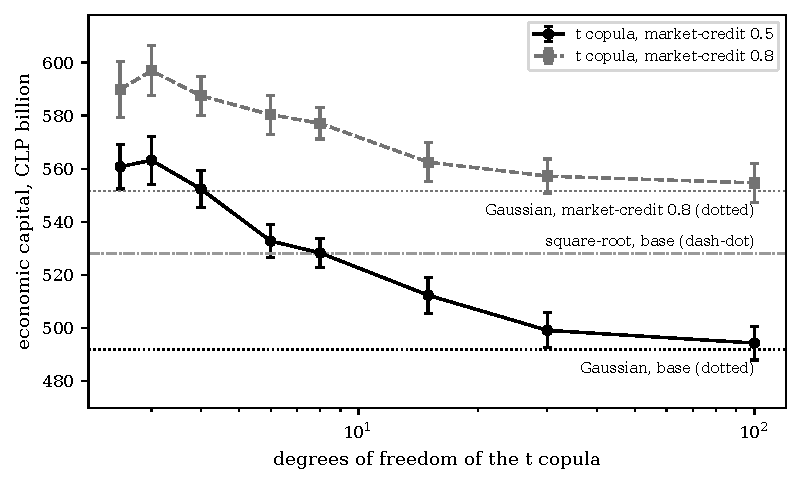
\includegraphics[width=0.82\textwidth]{figures/nu-curve}
\caption{The capital of the $t$ copula row against the degrees of freedom of the copula, in CLP billion, for the base matrix (solid) and for the matrix with market-credit correlation 0.8 (dashed), with two standard errors of each estimate from one run of $10^6$ draws. The dotted lines are the Gaussian copula row of each matrix and the dash-dotted line the square-root row of the base matrix.}
\label{fig:nu-curve}
\end{figure}

\subsection{Planted dependence structures}
\label{sec:results-planted}

Table~\ref{tab:planted-truth} and Figure~\ref{fig:truth-errors} set the rows of the band against the ten planted structures. The
capital of a structure ranges from CLP \bdTruthMin{} billion for independent risks to CLP \bdTruthMax{} billion for the $t$ copula with 3
degrees of freedom and the crisis matrix, which is $\bdTruthMaxOverHeadline$ of the headline and $\bdTruthMaxOverWorst$ of the worst case. The
standard error of every capital is at most CLP \bdTruthSeMax{} billion.

\begin{table*}[htbp]
\centering
\small
\caption{Ten planted dependence structures on the marginals of Banco Andino: the capital of the structure in CLP billion with its standard error over independent samples, the relative error in percent of the Gaussian copula row, of the square-root row, of the hybrid quantile with the correlation of the structure and of the Gaussian copula with its rank correlation, and whether the interior rows (hull), the interior rows of both matrices (hull+s) and the sharp range from the lower bound to the worst case contain it.}
\label{tab:planted-truth}
\fitwidth{\begin{tabular}{lrrrrrccc}
\toprule
Planted structure & Capital & Gauss. & Sqrt & Hybrid & Gauss. rank & Hull & Hull+s & Range \\
\midrule
\relax Gaussian, base matrix & \relax 487.9 $\pm$ 0.65 & \relax +0.0 & \relax +8.2 & \relax +0.9 & \relax -0.7 & \relax yes & \relax yes & \relax yes \\
\relax Gaussian, market-credit 0.8 & \relax 551.1 $\pm$ 1.06 & \relax -11.4 & \relax -4.2 & \relax -3.7 & \relax -0.6 & \relax no & \relax yes & \relax yes \\
\relax Gaussian, crisis matrix & \relax 575.9 $\pm$ 0.67 & \relax -15.3 & \relax -8.3 & \relax -4.1 & \relax +0.3 & \relax no & \relax yes & \relax yes \\
\relax Gaussian, independent risks & \relax 348.8 $\pm$ 0.45 & \relax +39.9 & \relax +51.4 & \relax +3.0 & \relax -0.3 & \relax no & \relax no & \relax yes \\
\relax t copula, 3 degrees, base matrix & \relax 555.6 $\pm$ 0.78 & \relax -12.2 & \relax -5.0 & \relax -8.9 & \relax -12.2 & \relax no & \relax yes & \relax yes \\
\relax t copula, 2.5 degrees, base matrix & \relax 560.9 $\pm$ 0.76 & \relax -13.0 & \relax -5.9 & \relax -12.2 & \relax -12.9 & \relax no & \relax yes & \relax yes \\
\relax t copula, 3 degrees, crisis matrix & \relax 611.1 $\pm$ 0.56 & \relax -20.1 & \relax -13.6 & \relax -9.1 & \relax -6.2 & \relax no & \relax no & \relax yes \\
\relax Gaussian regimes, 5 percent crisis & \relax 493.7 $\pm$ 0.57 & \relax -1.1 & \relax +7.0 & \relax +1.4 & \relax -0.9 & \relax yes & \relax yes & \relax yes \\
\relax Clayton, reflected, same mean tau & \relax 583.2 $\pm$ 1.10 & \relax -16.3 & \relax -9.4 & \relax -17.5 & \relax -21.8 & \relax no & \relax yes & \relax yes \\
\relax Gumbel, same mean tau & \relax 577.0 $\pm$ 1.13 & \relax -15.4 & \relax -8.5 & \relax -17.7 & \relax -21.7 & \relax no & \relax yes & \relax yes \\
\bottomrule
\end{tabular}}
\end{table*}


\begin{figure}[htbp]
\centering
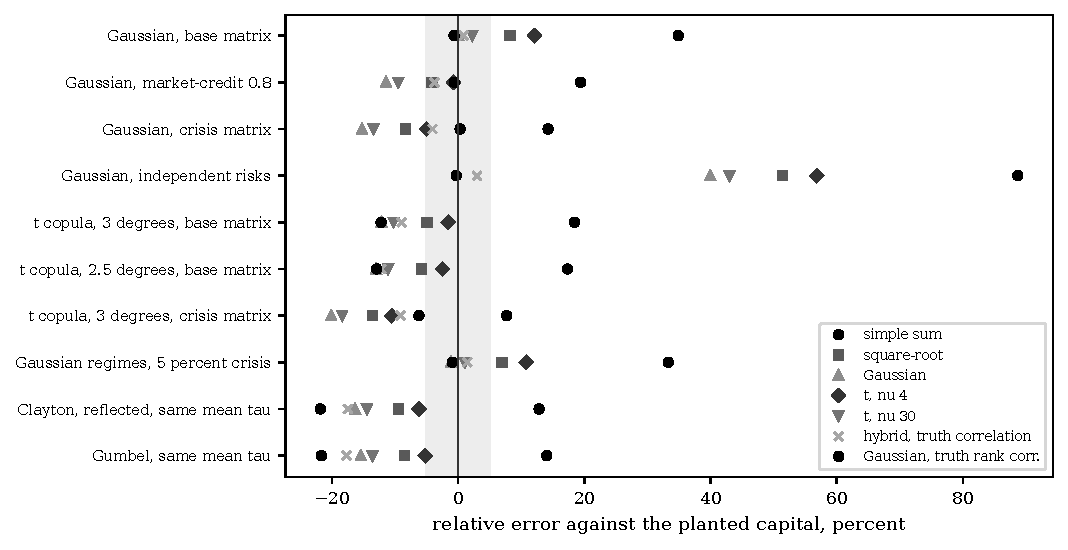
\includegraphics[width=0.92\textwidth]{figures/truth-errors}
\caption{Relative error in percent of six single-figure methods against the planted capital of each of the ten structures: the simple sum, the square-root row, the Gaussian copula row, the $t$ rows with 4 and 30 degrees of freedom, the hybrid quantile and the Gaussian copula calibrated on the structure itself. The shaded band marks errors within 5 percent; each marker is one method on one structure.}
\label{fig:truth-errors}
\end{figure}

\emph{Coverage by the sharp range (H4a).} The range from the lower bound to the worst case contains all $\bdCovSharp$ capitals,
which is Proposition~\ref{prop:coverage} met by the implementation. The range is wide: its median width is $\bdAblFullWidth$ times the
capital of the structure, and even the structure with the heaviest dependence is $\bdTruthMaxOverWorst$ of the worst case, so
the worst case is an outer bound and not a scenario.

\emph{Coverage by the interior rows (H4b, refuted).} The interval spanned by the five interior rows of the base matrix contains the
capital of $\bdCovInterior$ of the ten structures, the Gaussian copula with the base matrix, which is one of the rows, and the mixture
in which 95 percent of the draws follow it; the prediction required at least 75 percent. When the interior rows of the stressed
matrix are added, the interval contains $\bdCovInteriorStress$ of ten, and it misses independent risks, below the interval, and
the $t$ copula with 3 degrees of freedom and the crisis matrix, above it. The reflected Clayton copula is inside the interval, close to its upper end. The prediction on the interior rows alone is refuted; what the
interior rows cover depends on the matrix that is among them.

\emph{A single figure is not reliable (H4c).} The Gaussian row is within 5 percent of the capital in $\bdGaussWithin$ of the ten
structures, the structure that is Gaussian with the base matrix, where it is exact, and the mixture. Its absolute error has a median
of $\bdGaussMedErr$ percent and a maximum of $\bdGaussMaxErr$ percent, for independent risks, and it underestimates every structure that
has more dependence than the base matrix: with relative errors of $\bdGaussErrGaussianStress$ percent for the stressed matrix and
$\bdGaussErrTthreeCrisis$ percent for the heavy $t$ structure. The simple sum overestimates every structure and by up to
$\bdSumMaxErr$ percent. The prediction held.

The two estimators calibrated on the structure itself are better and not good. The hybrid quantile has a median absolute error of
$\bdHybridMedErr$ percent and a maximum of $\bdHybridMaxErr$ percent, and the Gaussian copula with the rank correlation of the
structure has a median of $\bdKendallMedErr$ percent and a maximum of $\bdKendallMaxErr$ percent. The latter is within $\bdKGaussMax$ percent for
all four Gaussian structures and for the mixture, because the Gaussian copula is the right family there, and it underestimates by $\bdKTailMin$
to $\bdKTailMax$ percent the $t$ and the two non-elliptical structures, whose tail dependence a matrix of rank correlations cannot carry
(Proposition~\ref{prop:tails}). A bank with a long history and a perfect estimate of the matrix would still need the band.

\subsection{The common horizon and level}
\label{sec:results-level}

Reading the market marginal at 99 percent in place of 99.9 percent lowers its capital from CLP \bdEcMarket{} to
CLP \bdMarketEcNineNine{} billion, a change of $\bdMarketEcChange$ percent, and lowers the simple sum to CLP \bdSumMismatch{}
billion, a change of $\bdHeadlineChange$ percent: a headline that looks like an aggregate at 99.9 percent and mixes two levels (H6).
The consistency test returns red on that band, and also on a band in which one marginal is read at a ten-day horizon, and green on
the consistent one. The engine itself refuses the band with the unconverted capital: the capital of the market marginal does not match
its quantile function at the level of the band within the tolerance of 1 percent. The two defences are independent, the test on the
metadata and the refusal on the values, and the prediction held. The size of the effect is that of the arithmetic of the
quantiles: the market marginal has no expected loss and carries $\bdEcShareMarket$ percent of the sum of the capital figures, so a
change of $\bdMarketEcChange$ percent in its capital moves the sum by about $\bdEcShareMarket$ percent of that, which is the
$\bdHeadlineChange$ percent observed. A change of this size in the headline is not a small inconsistency, and the aggregate that
results has no meaning as a quantile of any loss.

\subsection{Allocation and model-risk measures}
\label{sec:results-allocation}

Table~\ref{tab:euler} and Figure~\ref{fig:euler} give the Euler allocation of the expected shortfall of the Gaussian copula
aggregate over $20$ seeds. The aggregate expected shortfall is CLP \bdEsTotalMean{} $\pm$ \bdEsTotalSd{} billion, which contains the
committed value of CLP \bdEsTotal{} billion, and the contributions add up to it with a relative gap of at most $\bdEulerMaxGap$ in every
seed. The shares of the four risk types are $\bdShareCredit\pm\bdShareSdCredit$, $\bdShareMarket\pm\bdShareSdMarket$,
$\bdShareIrrbb\pm\bdShareSdIrrbb$ and $\bdShareOperational\pm\bdShareSdOperational$ percent. The allocation by stand-alone expected
shortfall sums to CLP \bdSumStandaloneEs{} billion, $\bdStandaloneOver$ times the aggregate, and over-allocates to the operational risk in
particular, whose benefit of diversification by the Euler allocation is $\bdBenefitOperational$ percent against $\bdBenefitCredit$,
$\bdBenefitMarket$ and $\bdBenefitIrrbb$ percent for credit, market and interest rate risk.

\begin{table}[htbp]
\centering
\small
\caption{The Euler allocation of the expected shortfall of the Gaussian copula aggregate at 99.9 percent in CLP billion, as mean over independent seeds with the standard deviation of the share, against the stand-alone expected shortfall of each marginal, which sums to more than the aggregate; the benefit is one minus the contribution over the stand-alone figure.}
\label{tab:euler}
\fitwidth{\begin{tabular}{lrrrrr}
\toprule
Risk & Euler contribution & Share, percent & Stand-alone ES & Share, percent & Benefit, percent \\
\midrule
\relax credit & \relax 258.5 & \relax 36.7 $\pm$ 1.2 & \relax 346.9 & \relax 35.4 & \relax 25 \\
\relax market & \relax 276.7 & \relax 39.3 $\pm$ 1.3 & \relax 355.8 & \relax 36.3 & \relax 22 \\
\relax IRRBB & \relax 78.5 & \relax 11.2 $\pm$ 0.3 & \relax 106.4 & \relax 10.9 & \relax 26 \\
\relax operational & \relax 90.0 & \relax 12.8 $\pm$ 2.7 & \relax 171.1 & \relax 17.5 & \relax 47 \\
\relax sum & \relax 703.7 & \relax 100.0 & \relax 980.2 & \relax 100.0 & \relax -- \\
\bottomrule
\end{tabular}}
\end{table}


\begin{figure}[htbp]
\centering
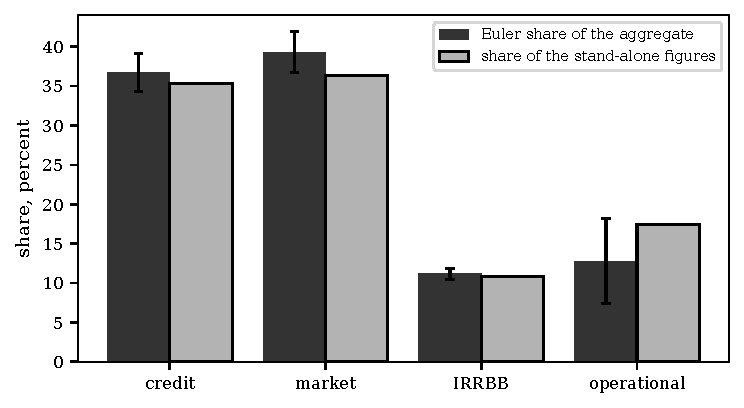
\includegraphics[width=0.7\textwidth]{figures/euler}
\caption{Share of each risk type in the aggregate expected shortfall of the Gaussian copula row at 99.9 percent: the Euler allocation (dark bars, mean over 20 seeds with two standard deviations) and the share in the sum of the stand-alone expected shortfalls (light bars), which does not describe the aggregate.}
\label{fig:euler}
\end{figure}

The model-risk measures of the band are information. With the Gaussian copula as the reference model, the additive measure is
$\bdAm$ percent and the relative measure is $\bdRm$: multiplying the Gaussian row by the factor $1+\mathrm{AM}$ reaches the worst
case, and the worst case lies above the Gaussian row by $\bdRmPct$ percent of the width of the band. The measure of Glasserman and Xu
with a relative entropy budget of $\bdGxEta$ raises the expected aggregate loss from CLP \bdGxBase{} to \bdGxWorst{} billion.

\subsection{The predictions}
\label{sec:results-hypotheses}

\begin{table}[htbp]
\centering
\small
\caption{The predictions stated before the experiments, the measured quantity of each and whether it held or was refuted, from the outputs of the experiment scripts.}
\label{tab:hypotheses}
\fitwidth{\begin{tabular}{llp{5.2cm}l}
\toprule
Id & Prediction & Measured & Outcome \\
\midrule
\relax H1 & \relax structure of the band in six committed aggregates & \relax 6 of 6 pass & \relax held \\
\relax H2 & \relax rebuilt rows reproduce the committed rows & \relax largest difference 0.0075 percent & \relax held \\
\relax H3 & \relax band wider than 100 standard errors; no row speaks for it & \relax width 205 s.e.; closest row 76 percent from another & \relax held \\
\relax H4a & \relax sharp range contains every planted capital & \relax 10 of 10 & \relax held \\
\relax H4b & \relax interior rows contain at least 75 percent of planted capitals & \relax 2 of 10 (8 with the stressed matrix) & \relax refuted \\
\relax H4c & \relax Gaussian row within 5 percent in at most half & \relax 2 of 10 & \relax held \\
\relax H5 & \relax bounds invariant to the matrix; Gaussian row moves over 10 percent & \relax bounds differ by 0; Gaussian row moves 12.1 percent & \relax held \\
\relax H6 & \relax level mismatch changes the sum over 10 percent and the test is red & \relax sum -17.9 percent; test red & \relax held \\
\relax H7 & \relax tests need the rows; Gaussian row alone runs at most half & \relax 6 of 9 run on the Gaussian row & \relax refuted \\
\bottomrule
\end{tabular}}
\end{table}


Table~\ref{tab:hypotheses} lists the outcome of each prediction. Seven of the nine held and two were refuted. The structure of the
rule (H1), the reproduction of the committed band (H2), the width of the band relative to its sampling error (H3), the coverage by
the sharp range (H4a), the weakness of a single Gaussian figure (H4c), the invariance of the bounds (H5) and the effect of an
unconverted level (H6) held. The coverage of the planted structures by the interior rows of the base matrix (H4b) was refuted,
with 2 of 10 against the 75 percent predicted, and the second clause of the prediction on the tests (H7) was refuted: six of the
nine tests, not at most half, can be run on the Gaussian row alone (Section~\ref{sec:ablation}). The two refuted predictions
concern the interior rows and the tests, not the structure of the rule or the reproduction of the band; Section~\ref{sec:discussion-failures}
discusses them. The measured column of the table keeps the units of the thresholds, so that a margin can be read: the width is
\bdWidthOverSe{} standard errors against 100, the Gaussian row moves $\bdGaussMove$ percent against 10, and the level mismatch moves the
sum by $\bdHeadlineChange$ percent against 10.

\section{Ablation}
\label{sec:ablation}

The ablation removes one component of the protocol at a time and measures what is lost on the ten planted structures of
Section~\ref{sec:design-planted}. Table~\ref{tab:ablation} gives every variant and Figure~\ref{fig:coverage} the counts of the
first nine. The components are the sharp bounds, the second matrix, the $t$ rows, the single figures that the band replaces, the
common level and the tests.

\begin{table*}[htbp]
\centering
\small
\caption{What each component of the protocol contributes on the ten planted structures: for an interval, the number of structures whose capital it contains and its median width relative to the capital; for a single figure, the number within the stated tolerance and its median absolute relative error.}
\label{tab:ablation}
\fitwidth{\begin{tabular}{p{5.6cm}lcrp{3.4cm}}
\toprule
Variant & Covered when & Structures covered & Median width / error & Missed \\
\midrule
\relax full band (bounds and all interior rows, base and stressed matrix) & \relax contains the capital & \relax 10 of 10 & \relax 1.26 & \relax none \\
\relax without the sharp bounds (interior rows, base and stressed matrix) & \relax contains the capital & \relax 8 of 10 & \relax 0.17 & \relax Gaussian, independent risks; t copula, 3 degrees, crisis matrix \\
\relax without the stressed matrix (interior rows of the base matrix) & \relax contains the capital & \relax 2 of 10 & \relax 0.11 & \relax covers only Gaussian, base matrix; Gaussian regimes, 5 percent crisis \\
\relax without the t copula rows (square-root rule and Gaussian copula, base matrix) & \relax contains the capital & \relax 2 of 10 & \relax 0.07 & \relax covers only Gaussian, base matrix; Gaussian regimes, 5 percent crisis \\
\relax without the t copula rows, with the stressed matrix (square-root rule and Gaussian copula, both matrices) & \relax contains the capital & \relax 5 of 10 & \relax 0.14 & \relax covers only Gaussian, base matrix; Gaussian, market-credit 0.8; t copula, 3 degrees, base matrix; t copula, 2.5 degrees, base matrix; Gaussian regimes, 5 percent crisis \\
\relax t copula rows only (4, 8 and 30 degrees of freedom, both matrices) & \relax contains the capital & \relax 6 of 10 & \relax 0.15 & \relax covers only Gaussian, market-credit 0.8; Gaussian, crisis matrix; t copula, 3 degrees, base matrix; t copula, 2.5 degrees, base matrix; Clayton, reflected, same mean tau; Gumbel, same mean tau \\
\relax Gaussian copula row alone & \relax within 5 percent & \relax 2 of 10 & \relax 0.14 & \relax median error \\
\relax square-root row alone & \relax within 5 percent & \relax 2 of 10 & \relax 0.08 & \relax median error \\
\relax simple sum alone (the headline) & \relax within 5 percent & \relax 0 of 10 & \relax 0.18 & \relax median error \\
\relax hybrid quantile with the correlation of the truth sample & \relax within 5 percent & \relax 5 of 10 & \relax 0.07 & \relax median error \\
\relax Gaussian copula with the rank correlation of the truth sample & \relax within 5 percent & \relax 5 of 10 & \relax 0.04 & \relax median error \\
\relax Gaussian copula alone, tolerance 10 percent & \relax within 10 percent & \relax 2 of 10 & \relax 0.14 & \relax median error \\
\bottomrule
\end{tabular}}
\end{table*}


\begin{figure}[htbp]
\centering
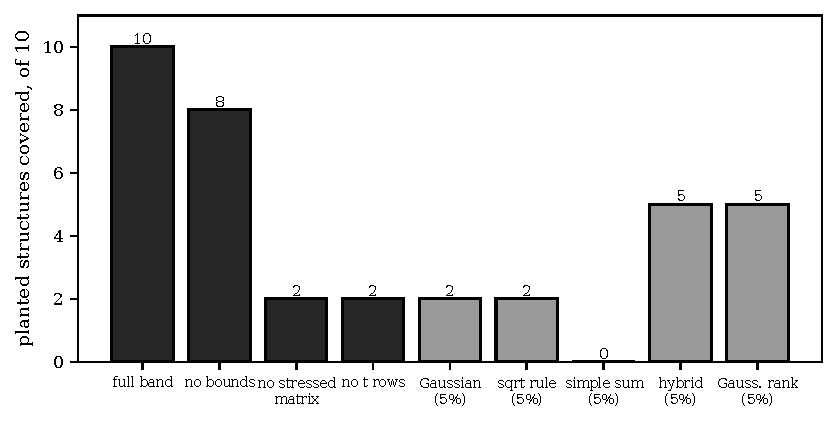
\includegraphics[width=0.9\textwidth]{figures/coverage}
\caption{Number of the ten planted structures covered by each variant: the full band and three intervals with one component removed (dark bars, containing the capital after widening by three standard errors), and five single figures (light bars, within 5 percent of the capital).}
\label{fig:coverage}
\end{figure}

\subsection{Components of the band read as an interval}
\label{sec:ablation-intervals}

The full band, with the bounds and the interior rows of both matrices, contains all ten capitals and has a median width of
$\bdAblFullWidth$ times the capital. Removing the sharp bounds leaves an interval of median width $\bdAblNoBoundsWidth$ that contains
$\bdAblNoBounds$ of the ten: it misses \bdMissedNoBounds{}, the structure with no dependence, which lies below every interior row, and
the heaviest tail, which lies above every interior row. The bounds therefore buy the last $\bdAblBoundsGain$ structures at a price of $\bdAblWidthBounds$ of the capital in median width, which is a high
price and a necessary one if coverage is the goal: no
choice of copula family and matrix can be known to span the structures that were not thought of, and the bounds are the only
rows that do not depend on that choice.

The stressed matrix is the component with the highest value for its width. Without it the interior rows of the base matrix
contain $\bdAblNoStress$ of the ten structures with a median width of $\bdAblNoStressWidth$; with it, and without the bounds, they
contain $\bdAblNoBounds$ at $\bdAblNoBoundsWidth$. The increase of $\bdAblStressGain$ structures costs $\bdAblWidthStress$ of the capital in median width. The $t$ rows have
the opposite profile on the base matrix: removing them leaves the square-root rule and the Gaussian row, which contain
$\bdAblNoT$ of the ten at a width of $\bdAblNoTWidth$, the same count as the five-row interval of the base matrix. Their
contribution appears in combination with the stressed matrix: without the $t$ rows but with both matrices the interval contains
$\bdAblNoTStress$ of the ten at a median width of $\bdAblNoTStressWidth$, against $\bdAblNoBounds$ for the five interior rows of
both matrices, and the $t$ rows alone, on both matrices, contain $\bdAblTOnly$ at $\bdAblTOnlyWidth$. The three components are
not additive, because each interior interval extends the others in different directions: the matrix moves the Gaussian
structures up, the $t$ rows move the capital of the heavy-tailed structures up, and neither can reach the independent case, which
only the bounds contain.

\subsection{Single figures against the band}
\label{sec:ablation-single}

A single figure is the alternative that the band replaces. Used alone and with a tolerance of 5 percent, the Gaussian copula row
is within the tolerance of $\bdAblGaussPoint$ of the ten structures, the square-root row of $\bdAblVcPoint$, the simple sum of
$\bdAblSumPoint$, the hybrid quantile calibrated on the structure of $\bdAblHybridPoint$ and the Gaussian copula calibrated on its rank
correlation of $\bdAblKendallPoint$. Loosening the tolerance of the Gaussian row to 10 percent does not change its count,
$\bdAblGaussTen$, because its errors are either below 2 percent or above 11 percent. The row that scores best as a point estimate when it
is calibrated on the structure, the Gaussian copula with the rank correlation of the structure, fails exactly on the structures
that Proposition~\ref{prop:tails} predicts it fails on, the five whose dependence has tail dependence, and the cost of that
failure is an underestimate of $\bdKTailMin$ to $\bdKTailMax$ percent. The interval is more informative than any of these figures because it states the
width of what is not known, and the width is the quantity that the single figures conceal: even the best calibrated estimator,
with a median error of $\bdKendallMedErr$ percent, has no indication of the 22 percent that it misses on the worst structure.
The comparison is conservative against the band, because the band's interior rows use named conventions while the competing
estimators use the structure's own data.

\subsection{The tests that each row feeds}
\label{sec:ablation-tests}

The tests of Section~\ref{sec:method-checks} each read a defined set of inputs, listed in Table~\ref{tab:tests-rows}. Removing the
$t$ rows leaves the copula-choice test unrunnable: the engine returns the light not evaluated when it is given an empty list of
$t$ capital figures. The correlation-stress test needs the Gaussian row of the stressed matrix, and the bracket test needs the two
bound rows, so removing the stressed band or the bounds leaves each without its input; these two are determined by the arguments
of the functions, which take the missing row as a required argument, and not by an engine call that refuses them. The first clause
of the prediction (H7) holds on these grounds.

\begin{table}[htbp]
\centering
\small
\caption{The nine tests of the aggregation battery, the rows or inputs each one reads, the light each returns on the committed aggregate and whether the test can be run when the Gaussian copula row is the only aggregate figure kept; the two amber lights belong to tests that read more than one row.}
\label{tab:tests-rows}
\fitwidth{\begin{tabular}{p{4.4cm}p{5.6cm}ll}
\toprule
Test of the aggregation battery & Inputs it reads & Light on the committed aggregate & Runs on the Gaussian row alone \\
\midrule
\relax simple sum and variance covariance & \relax Gaussian row; marginal capitals; correlation matrix & \relax green & \relax yes \\
\relax copula choice sensitivity & \relax Gaussian row; t rows & \relax amber & \relax no \\
\relax worst case bracket & \relax lower bound; worst case; interior rows & \relax green & \relax no \\
\relax correlation stress & \relax Gaussian row of the base matrix; Gaussian row of the stressed matrix & \relax amber & \relax no \\
\relax diversification sign & \relax the diversification factor of each interior row & \relax green & \relax yes \\
\relax horizon confidence consistency & \relax horizon and level of each marginal & \relax green & \relax yes \\
\relax euler additivity & \relax the Euler contributions and the aggregate expected shortfall & \relax green & \relax yes \\
\relax elliptical mc agreement & \relax square-root row; an elliptical simulation & \relax green & \relax yes \\
\relax rosenberg schuermann reference & \relax simple sum; Gaussian row & \relax green & \relax yes \\
\bottomrule
\end{tabular}}
\end{table}


The second clause was refuted. With the Gaussian row as the only aggregate figure kept, $\bdRunnableGaussOnly$ of the
$\bdTestsTotal$ tests still run, not at most half: the comparison with the simple sum and the square-root rule, the sign of the
diversification factors, the consistency of the horizon and the level, the additivity of the allocation, the agreement of a
Monte Carlo run with the square-root rule, and the reference of Rosenberg and Schuermann read the Gaussian row, the marginals or
the conventions. The prediction was mistaken about the proportion, not about the mechanism: the three tests that read the other
rows are the three that measure the dependence uncertainty (the sensitivity to the copula, the stress of the matrix and the bracket
of the bounds), and the six that run on a Gaussian row alone are those that verify arithmetic, units and a reference. The tests of the
dependence uncertainty are the ones that fail without the band.

\subsection{The common level and the allocation}
\label{sec:ablation-level}

The two remaining components were ablated in Section~\ref{sec:results}. Reading one marginal at another level changes the headline by
$\bdHeadlineChange$ percent and is caught twice, by the consistency test and by the refusal of the engine. The Euler allocation is
compared with the allocation by stand-alone expected shortfall, which sums to $\bdStandaloneOver$ times the aggregate and so is not
an allocation of it; the Euler allocation adds up to the aggregate in every seed to a relative $\bdEulerMaxGap$, and its price is
a sampling standard deviation of $\bdShareSdMin$ to $\bdShareSdMax$ percentage points in a share, because it rests on the same thousand tail draws as the
value at risk. Neither ablation changes a row of the band: the level check protects the inputs and the allocation extends the
output. Their value is that they close two routes by which a correct band can be misread, a headline built from marginals at
different levels, which no row would reveal because every row inherits it, and an allocation whose parts do not sum to the whole,
which a reader would otherwise normalise by eye. The refusal of the engine for an unconverted capital is the stronger of the two
defences on the level, since it holds when the metadata of the marginals are wrong.

\section{Discussion}
\label{sec:discussion}

\subsection{Why the band looks the way it does}
\label{sec:discussion-why}

The band of Banco Andino spans the interval from $\bdLowerDf$ to $\bdWorstDf$ of the headline, and the two ends are far from
everything that a plausible dependence produces. The largest capital among the ten planted structures is $\bdTruthMaxOverHeadline$
of the headline, reached by a $t$ copula with 3 degrees of freedom and a crisis matrix, and the worst case is $\bdWorstDf$.
The reason is in the construction of the sharp bounds. The worst case moves the largest losses of each risk type into the
scenarios where the other types have small ones, so that every scenario of the tail has nearly the same total
(Figure~\ref{fig:rearrangement}); no positive dependence structure does that, and it is the structure that makes the value at risk
exceed the sum of the values at risk by $\bdWorstOverComo$ percent. It is a bound that states what cannot be excluded without
knowledge of the dependence, and the planted structures confirm that it is not a scenario. The lower bound is the mirror image, a
structure in which the large losses never coincide, and the independent risks, at $\bdTruthDfGaussianIndependent$ of the
headline, are still far above it.

The interior rows describe the plausible structures, and what they cover is decided by the matrices. With the base matrix alone the
five interior rows contain two of the ten structures; with the stressed matrix added they contain eight, and the interval grows
by $\bdAblWidthStress$ of the capital. The matrix, not the family, is the first-order component, and Proposition~\ref{prop:sqrt}
shows why for the square-root row: the effect of a correlation is the product of the two capital figures, so the pair of the largest
marginals, credit and market, carries most of the movement. The family matters in a second order, through the tail dependence that
Proposition~\ref{prop:tails} describes, and the experiment with the planted structures shows the order of magnitude: a Gaussian
copula calibrated on the exact rank correlation of the structure is within $\bdKGaussMax$ percent for the five Gaussian-family structures and
\bdKTailMin{} to \bdKTailMax{} percent below for the five with tail dependence.

\subsection{Failure cases and negative results}
\label{sec:discussion-failures}

Two predictions were refuted and both are informative. The interior rows of the base matrix covered 2 of the 10 structures
against the 75 percent predicted. The prediction assumed that the interior rows, which are five different aggregation
methods, would bracket the plausible structures; in fact they bracket the plausible structures only when the matrix is right. A
validator that reads the base band alone concludes that the aggregate is between CLP \bdGauss{} and \bdTFour{} billion (the Gaussian
row to the $t$ row of 4 degrees of freedom), and eight of the ten planted structures, which a bank may
reasonably worry about, lie outside that interval. The stress matrix makes the difference. This is a finding about the protocol:
the band must carry the stressed matrix as a first-class component, which the rule of Section~\ref{sec:method-rule} does by naming
the matrices as conventions of the same document.

The second refutation, that more than half of the tests run on the Gaussian row alone, shows that the number of tests is not the
measure of the protection that the band offers. Six tests verify arithmetic, units, consistency and a reference and run on any
single row. The three that read the other rows are the ones that measure the dependence uncertainty, and those fail without the band.
The refutation also gives a use for the table of Section~\ref{sec:ablation-tests}: it says which tests are protections against a
single-figure report.

Three other limits of the results are negative in a milder sense. The additivity of the Euler allocation holds to
$\bdEulerMaxGap$ because it is an identity of the estimator; the test guards the implementation, and the information in the allocation
is its sampling error, which has a standard deviation of $\bdShareSdMax$ percentage points for operational risk. The hypothesis that the sharp range
covers every planted structure was predicted correctly and carries no information about the structures, as
Proposition~\ref{prop:coverage} shows. And the $t$ curve is flat between 2.5 and 3 degrees of freedom within the noise, so the
conjecture of monotonicity is supported on a grid that has one flat step.

\subsection{What the band lets a validator say}
\label{sec:discussion-validator}

The band changes the form of the statement that a validator can make about an aggregate. Without it, the statement is that the
aggregate is a figure from a method with a matrix. With it, the validator can say what share of the width belongs to the choice of
method (the Gaussian and the $t$ rows differ by up to $\bdCopulaDiffFour$ percent, amber in the copula test), what share to
the matrix (the stress moves the Gaussian row by $\bdGaussMove$ percent, amber in the stress test), and what share to the
dependence that no copula of the set spans (the distance from the interior rows to the bounds). The model-risk measures of the band
put numbers on the same: $\mathrm{AM}$ of $\bdAm$ percent says that the worst case is $\bdAm$ percent above the Gaussian figure,
and $\mathrm{RM}$ of $\bdRm$ places it within the band.

The findings also bear on what a bank should report as capital. The case keeps the simple sum as the headline, on the supervisory
position that diversification between risk types is not recognised; the experiments show that the position is conservative for
every planted structure with positive dependence, since the simple sum exceeds the capital of each by $\bdSumErrMin$ to $\bdSumErrMaxOther$ percent, except for
the independent structure, where it exceeds it by $\bdSumMaxErr$ percent. A bank that did claim diversification would have to
choose one row of the band, and the experiments give it a reason for the choice: the Gaussian row underestimates by $\bdGaussDepMin$ to $\bdGaussDepMax$ percent
every planted structure with a stressed matrix or with tail dependence, seven of the ten, and the interior rows of the stressed matrix come closer: on these seven structures the Gaussian row of the stressed matrix falls short by
$\bdGaussStressDepMin$ to $\bdGaussStressDepMax$ percent, against $\bdGaussDepMin$ to $\bdGaussDepMax$ percent below for the Gaussian row of the base matrix.

\subsection{Relation to the published findings}
\label{sec:discussion-literature}

The overestimate of the additive rule over the Gaussian copula in the case, $\bdAdditiveOver$ percent, lies in the range of 30 to 40
percent that Rosenberg and Schuermann report \citep{rosenberg2006}. The same authors find that the choice between a normal and a Student $t$ copula has a more modest effect
on risk than the additive overestimate; the case agrees in order of magnitude, since the largest difference between a $t$ row and
the Gaussian row is $\bdCopulaStat$ percent, against $\bdAdditiveOver$ percent for the simple sum. The excess of the worst value at risk over the comonotonic one,
$\bdWorstOverComo$ percent here, is the phenomenon that Embrechts, Puccetti and R\"uschendorf describe and that makes the simple
sum a non-bound \citep{epr2013}. The dependence of the capital on the degrees of freedom is that of the tail dependence of
Demarta and McNeil \citep{demarta2005}. The Joint Forum's reluctance to rely on aggregation models \citep{jointforum2010} is, in
these numbers, a reluctance to rely on one row: the band of a single case shows that the figures of the rows differ by amounts
that no supervisor can ignore. None of these is a new finding. What the experiments add is the measurement of what the band contains
when the structure is known, and the identification of the matrix as the component that decides it.

\section{Limitations}
\label{sec:limitations}

\subsection{Internal validity}
\label{sec:limits-internal}

The simulated rows are sample quantiles at 99.9 percent from $10^6$ draws, so each rests on 1,000 tail draws, and their standard
errors are about one percent of a row. The comparisons that matter are two orders of magnitude larger than this error (the width
of the band is \bdWidthOverSe{} standard errors), but the coverage of a structure whose capital lies within a few standard errors of
the edge of an interval is sensitive to it: the reflected Clayton copula is inside the interval of both matrices near its upper end,
and a different seed could move it across. The widening by three standard errors of the capital of the structure, the tolerance of
5 percent, the 75 percent of the coverage and the 100 standard errors of the width are thresholds of the author, fixed before the
experiments and not derived. The capital of a planted structure is itself an estimate, from 20 samples of $10^6$ draws, with a
standard error of at most CLP \bdTruthSeMax{} billion. The rearrangement algorithm that computes the bounds has no proof of
convergence; the evidence here is the narrowness of the ranges, and a marginal with another shape of tail could behave otherwise.
The coverage of the planted structures by the sharp range is, by Proposition~\ref{prop:coverage}, a check of the implementation and
not a finding. The classification of a test as unrunnable without a row is made by the arguments of the function for two of the
tests and by an engine call for one.

\subsection{External validity}
\label{sec:limits-external}

All results are for one synthetic bank, four risk types, one level of 99.9 percent and one horizon of one year. The marginals are
simulated by the producers of the case, and two of them rest on conventions that the case records as conventions: the
market marginal is moved from 99 percent and one day to 99.9 percent and one year by the normal quantile ratio and the square root
of 250, and the correlation of interest rate risk with the other types is set equal to that of market risk, which the case records as unverified. Each moves every row
of the band alike, so the band does not remove it; the band shows the dependence uncertainty conditional on the marginals and not
the uncertainty of the marginals. The marginals are read from a grid of $\bdGridPoints$ probabilities that ends at $5\times10^{-7}$ on each
side with linear interpolation and clamping, so the rearrangement for the worst case reads the quantile functions only as far as
the grid allows; the lower end of the grid reaches losses of CLP \bdMarketGridMin{} billion for the market marginal, and a bound row
that depends on the extreme tail beyond the grid would not see it. The ten planted structures are chosen by the author, include
several that are in the family of the band, and are not a sample of the dependence structures of banks: the proportions covered
are properties of this set. The competing single-figure estimators were calibrated on data of the planted structure, which is
favourable to them, and the band's interior rows use named conventions; with real data a bank would have a noisier matrix.

\subsection{Construct validity}
\label{sec:limits-construct}

The experiments measure coverage of the capital of planted structures with the marginals of the case, so they measure whether the
band brackets the effect of the dependence on the capital, which is the construct of the dependence band. They do not measure
whether the band is useful for a decision, whether it changes what a bank holds, or whether a supervisor would accept it. The
width is used as the price of coverage, and a more informative comparison would be a proper scoring rule for an interval, which
is not computed here. The planted structures share the marginals of the case, so a structure that changes the marginals, such as a
dependence between the frequency and the severity of operational losses, is outside what they test; the band is conditional on
the marginals by design. The Euler allocation is evaluated for the expected shortfall of the Gaussian copula row only, and the
model-risk measures are computed on the band of that one aggregate; neither is validated against a known allocation or a known
model risk.

\subsection{Scope}
\label{sec:limits-scope}

The study does not claim that the band is optimal, that no other interval construction is better, or that the band's rows are the
only ones that a validator should show; the bounds with a constraint on the variance of the sum \citep{brv2015}, for example, give
narrower intervals under extra information and are not run here. It does not claim that no maintained toolkit or published practice
reports the band beside every aggregate, since no search beyond the cited sources was made. It does not examine the aggregation of
the expected shortfall, only of the value at risk at one level, nor a number of risk types other than four. The acceptance criteria
of the tests are internal to the validation, and no result is a statement about regulatory compliance. Nor does it claim that eight
is the right number of rows: the set of degrees of freedom is a convention, and a set with another number of values gives a band
with more or fewer rows under the same rule, so the claim is about the rule and the number of rows follows from the set.

\section{Reproducibility}
\label{sec:reproducibility}

The source of the manuscript, the experiment scripts and their outputs are in the repository of the case, under
\texttt{manuscripts/dependence-band-with-every-aggregate}, and the data are the committed documents under
\texttt{data/derived/C18}. The engine is \texttt{riskvalidation} 1.1.0 with its market, machine-learning and stress extras,
installed in an environment of the repository's pipeline requirements; the figure and table scripts use the shared kit
\texttt{manuscripts/\_shared/figkit.py}. No experiment reads data outside the repository, and none needs network access. The
commands below name the scripts relative to the manuscript folder, and each is run with the interpreter of that environment; the
scripts locate the repository root themselves.

\begin{enumerate}
\item \texttt{python experiments/e1\_structure.py}: the structure of the six
committed aggregates, the closed-form checks and the analytic ceiling (about 4 seconds).
\item \texttt{python experiments/e2\_reproduce.py}: the reproduction at the
committed seed, the 20 and 10 independent bands, the rearrangement ranges and the $t$ curve (about 9 minutes).
\item \texttt{python experiments/e3\_planted\_truth.py}: the ten planted
structures with 20 samples each and the two calibrated comparators (about 9 minutes; it reads the output of the second script).
\item \texttt{python experiments/e4\_ablation.py}: the level mismatch, the tests,
the Euler allocation over 20 seeds and the ablation variants (under one minute; it reads the output of the third).
\item \texttt{python experiments/e5\_timing.py}: the run time of one band and of its bound rows (under one minute).
\item \texttt{python make\_artifacts.py}: the seven figures, the nine tables and the
file of number macros that the text reads (under one minute).
\end{enumerate}

Each experiment writes a compact JSON file beside its script, and the figure and table script reads only those files and the
committed documents, so a number of the text is regenerated by its script and never typed. The predictions are in
\texttt{experiments/hypotheses.json}, read by the scripts, and their criteria are not edited after a run. The seeds are fixed in the
scripts and listed in Section~\ref{sec:design-statistics}: re-running the scripts reproduces every stored number
exactly. The
references are rebuilt by \texttt{fetch\_references.py}, which retrieves each record from its DOI. The run times are those of one
workstation with a single process per script. The text is built with \texttt{pdflatex} and \texttt{bibtex}, two further passes of
\texttt{pdflatex}, in a folder outside the repository.

\section{Conclusions}
\label{sec:conclusions}

A rule that reports every aggregate capital figure with a band of eight rows over the same marginals, one horizon and one level,
with one headline and seven rows labelled information, can be implemented, checked and reproduced: the six committed aggregates of
the case satisfy it, the engine rebuilds the committed rows from the committed marginal grids to within \bdMaxRelDiff{} percent,
and the band of Banco Andino runs from CLP \bdLower{} to \bdWorst{} billion against a headline of CLP \bdHeadline{} billion, which
is \bdWidthOverSe{} Monte Carlo standard errors wide.

On ten planted dependence structures of known capital, the sharp range contains all of them, at a median width of
$\bdAblFullWidth$ times the capital, which is a property of the bounds and not of the structures. The interior rows of the base
matrix contain $\bdCovInterior$ of the ten, against the 75 percent that was predicted, and $\bdCovInteriorStress$ when the rows of the
stressed matrix are added: the matrix is the component that decides what the interior rows cover. The Gaussian copula row alone is
within 5 percent of the capital of $\bdGaussWithin$ structures, with a median error of $\bdGaussMedErr$ percent, and two
single-figure estimators calibrated on the structure itself are within 5 percent in $\bdAblHybridPoint$ of the ten. The tail dependence
that a correlation matrix does not carry is the reason, and the band shows it. The Euler allocation adds up to
the aggregate by construction, and the tests that need rows beyond the Gaussian one are the three that measure the dependence
uncertainty.

The next steps are three. The band should be evaluated on aggregates whose marginals are not simulated by the same producer, so
that the effect of a marginal error on the rows can be separated from the dependence uncertainty. The interior of the band should
be enriched with families that carry tail dependence in the loss direction, such as the Clayton and Gumbel copulas that the study
planted, to test whether the coverage of the interior rows then reaches the level that was predicted. And the intervals that
use additional information, such as a constraint on the variance of the sum, should be run on the same marginals and compared with
the band at equal coverage, which is the comparison that the present study did not make.


\bibliographystyle{plainnat}
\bibliography{references}

\end{document}
